% Options for packages loaded elsewhere
\PassOptionsToPackage{unicode}{hyperref}
\PassOptionsToPackage{hyphens}{url}
%
\documentclass[
]{book}
\usepackage{amsmath,amssymb}
\usepackage{lmodern}
\usepackage{iftex}
\ifPDFTeX
  \usepackage[T1]{fontenc}
  \usepackage[utf8]{inputenc}
  \usepackage{textcomp} % provide euro and other symbols
\else % if luatex or xetex
  \usepackage{unicode-math}
  \defaultfontfeatures{Scale=MatchLowercase}
  \defaultfontfeatures[\rmfamily]{Ligatures=TeX,Scale=1}
\fi
% Use upquote if available, for straight quotes in verbatim environments
\IfFileExists{upquote.sty}{\usepackage{upquote}}{}
\IfFileExists{microtype.sty}{% use microtype if available
  \usepackage[]{microtype}
  \UseMicrotypeSet[protrusion]{basicmath} % disable protrusion for tt fonts
}{}
\makeatletter
\@ifundefined{KOMAClassName}{% if non-KOMA class
  \IfFileExists{parskip.sty}{%
    \usepackage{parskip}
  }{% else
    \setlength{\parindent}{0pt}
    \setlength{\parskip}{6pt plus 2pt minus 1pt}}
}{% if KOMA class
  \KOMAoptions{parskip=half}}
\makeatother
\usepackage{xcolor}
\IfFileExists{xurl.sty}{\usepackage{xurl}}{} % add URL line breaks if available
\IfFileExists{bookmark.sty}{\usepackage{bookmark}}{\usepackage{hyperref}}
\hypersetup{
  pdftitle={Advanced R Exercises},
  pdfauthor={Indrajeet Patil},
  hidelinks,
  pdfcreator={LaTeX via pandoc}}
\urlstyle{same} % disable monospaced font for URLs
\usepackage{color}
\usepackage{fancyvrb}
\newcommand{\VerbBar}{|}
\newcommand{\VERB}{\Verb[commandchars=\\\{\}]}
\DefineVerbatimEnvironment{Highlighting}{Verbatim}{commandchars=\\\{\}}
% Add ',fontsize=\small' for more characters per line
\usepackage{framed}
\definecolor{shadecolor}{RGB}{248,248,248}
\newenvironment{Shaded}{\begin{snugshade}}{\end{snugshade}}
\newcommand{\AlertTok}[1]{\textcolor[rgb]{0.94,0.16,0.16}{#1}}
\newcommand{\AnnotationTok}[1]{\textcolor[rgb]{0.56,0.35,0.01}{\textbf{\textit{#1}}}}
\newcommand{\AttributeTok}[1]{\textcolor[rgb]{0.77,0.63,0.00}{#1}}
\newcommand{\BaseNTok}[1]{\textcolor[rgb]{0.00,0.00,0.81}{#1}}
\newcommand{\BuiltInTok}[1]{#1}
\newcommand{\CharTok}[1]{\textcolor[rgb]{0.31,0.60,0.02}{#1}}
\newcommand{\CommentTok}[1]{\textcolor[rgb]{0.56,0.35,0.01}{\textit{#1}}}
\newcommand{\CommentVarTok}[1]{\textcolor[rgb]{0.56,0.35,0.01}{\textbf{\textit{#1}}}}
\newcommand{\ConstantTok}[1]{\textcolor[rgb]{0.00,0.00,0.00}{#1}}
\newcommand{\ControlFlowTok}[1]{\textcolor[rgb]{0.13,0.29,0.53}{\textbf{#1}}}
\newcommand{\DataTypeTok}[1]{\textcolor[rgb]{0.13,0.29,0.53}{#1}}
\newcommand{\DecValTok}[1]{\textcolor[rgb]{0.00,0.00,0.81}{#1}}
\newcommand{\DocumentationTok}[1]{\textcolor[rgb]{0.56,0.35,0.01}{\textbf{\textit{#1}}}}
\newcommand{\ErrorTok}[1]{\textcolor[rgb]{0.64,0.00,0.00}{\textbf{#1}}}
\newcommand{\ExtensionTok}[1]{#1}
\newcommand{\FloatTok}[1]{\textcolor[rgb]{0.00,0.00,0.81}{#1}}
\newcommand{\FunctionTok}[1]{\textcolor[rgb]{0.00,0.00,0.00}{#1}}
\newcommand{\ImportTok}[1]{#1}
\newcommand{\InformationTok}[1]{\textcolor[rgb]{0.56,0.35,0.01}{\textbf{\textit{#1}}}}
\newcommand{\KeywordTok}[1]{\textcolor[rgb]{0.13,0.29,0.53}{\textbf{#1}}}
\newcommand{\NormalTok}[1]{#1}
\newcommand{\OperatorTok}[1]{\textcolor[rgb]{0.81,0.36,0.00}{\textbf{#1}}}
\newcommand{\OtherTok}[1]{\textcolor[rgb]{0.56,0.35,0.01}{#1}}
\newcommand{\PreprocessorTok}[1]{\textcolor[rgb]{0.56,0.35,0.01}{\textit{#1}}}
\newcommand{\RegionMarkerTok}[1]{#1}
\newcommand{\SpecialCharTok}[1]{\textcolor[rgb]{0.00,0.00,0.00}{#1}}
\newcommand{\SpecialStringTok}[1]{\textcolor[rgb]{0.31,0.60,0.02}{#1}}
\newcommand{\StringTok}[1]{\textcolor[rgb]{0.31,0.60,0.02}{#1}}
\newcommand{\VariableTok}[1]{\textcolor[rgb]{0.00,0.00,0.00}{#1}}
\newcommand{\VerbatimStringTok}[1]{\textcolor[rgb]{0.31,0.60,0.02}{#1}}
\newcommand{\WarningTok}[1]{\textcolor[rgb]{0.56,0.35,0.01}{\textbf{\textit{#1}}}}
\usepackage{longtable,booktabs,array}
\usepackage{calc} % for calculating minipage widths
% Correct order of tables after \paragraph or \subparagraph
\usepackage{etoolbox}
\makeatletter
\patchcmd\longtable{\par}{\if@noskipsec\mbox{}\fi\par}{}{}
\makeatother
% Allow footnotes in longtable head/foot
\IfFileExists{footnotehyper.sty}{\usepackage{footnotehyper}}{\usepackage{footnote}}
\makesavenoteenv{longtable}
\usepackage{graphicx}
\makeatletter
\def\maxwidth{\ifdim\Gin@nat@width>\linewidth\linewidth\else\Gin@nat@width\fi}
\def\maxheight{\ifdim\Gin@nat@height>\textheight\textheight\else\Gin@nat@height\fi}
\makeatother
% Scale images if necessary, so that they will not overflow the page
% margins by default, and it is still possible to overwrite the defaults
% using explicit options in \includegraphics[width, height, ...]{}
\setkeys{Gin}{width=\maxwidth,height=\maxheight,keepaspectratio}
% Set default figure placement to htbp
\makeatletter
\def\fps@figure{htbp}
\makeatother
\setlength{\emergencystretch}{3em} % prevent overfull lines
\providecommand{\tightlist}{%
  \setlength{\itemsep}{0pt}\setlength{\parskip}{0pt}}
\setcounter{secnumdepth}{5}
\usepackage{booktabs}
\ifLuaTeX
  \usepackage{selnolig}  % disable illegal ligatures
\fi
\usepackage[]{natbib}
\bibliographystyle{apalike}

\title{Advanced R Exercises}
\author{Indrajeet Patil}
\date{2022-02-07}

\begin{document}
\maketitle

{
\setcounter{tocdepth}{1}
\tableofcontents
}
\hypertarget{about}{%
\chapter*{About}\label{about}}
\addcontentsline{toc}{chapter}{About}

My solutions to exercises from Hadley Wickham's \emph{Advanced R} book:

\url{https://adv-r.hadley.nz/}

For the official solution manual, see:

\url{https://advanced-r-solutions.rbind.io/}

\hypertarget{part-foundations}{%
\part{Foundations}\label{part-foundations}}

\hypertarget{names-and-values}{%
\chapter{Names and values}\label{names-and-values}}

\hypertarget{exercises}{%
\section{2.2.2 Exercises}\label{exercises}}

\hypertarget{q1.-explain-the-relationship}{%
\subsection*{Q1. Explain the relationship}\label{q1.-explain-the-relationship}}
\addcontentsline{toc}{subsection}{Q1. Explain the relationship}

\begin{Shaded}
\begin{Highlighting}[]
\NormalTok{a }\OtherTok{\textless{}{-}} \DecValTok{1}\SpecialCharTok{:}\DecValTok{10}
\NormalTok{b }\OtherTok{\textless{}{-}}\NormalTok{ a}
\NormalTok{c }\OtherTok{\textless{}{-}}\NormalTok{ b}
\NormalTok{d }\OtherTok{\textless{}{-}} \DecValTok{1}\SpecialCharTok{:}\DecValTok{10}
\end{Highlighting}
\end{Shaded}

All of these variable names are actively bound to the same value.

\begin{Shaded}
\begin{Highlighting}[]
\FunctionTok{library}\NormalTok{(lobstr)}

\FunctionTok{obj\_addr}\NormalTok{(a)}
\CommentTok{\#\textgreater{} [1] "0x14bc0998"}
\FunctionTok{obj\_addr}\NormalTok{(b)}
\CommentTok{\#\textgreater{} [1] "0x14bc0998"}
\FunctionTok{obj\_addr}\NormalTok{(c)}
\CommentTok{\#\textgreater{} [1] "0x14bc0998"}
\FunctionTok{obj\_addr}\NormalTok{(d)}
\CommentTok{\#\textgreater{} [1] "0x16c543b8"}
\end{Highlighting}
\end{Shaded}

\hypertarget{q2.-function-object-address}{%
\subsection*{Q2. Function object address}\label{q2.-function-object-address}}
\addcontentsline{toc}{subsection}{Q2. Function object address}

Following code verifies that indeed these calls all point to the same underlying function object.

\begin{Shaded}
\begin{Highlighting}[]
\FunctionTok{obj\_addr}\NormalTok{(mean)}
\CommentTok{\#\textgreater{} [1] "0x1653eaf0"}
\FunctionTok{obj\_addr}\NormalTok{(base}\SpecialCharTok{::}\NormalTok{mean)}
\CommentTok{\#\textgreater{} [1] "0x1653eaf0"}
\FunctionTok{obj\_addr}\NormalTok{(}\FunctionTok{get}\NormalTok{(}\StringTok{"mean"}\NormalTok{))}
\CommentTok{\#\textgreater{} [1] "0x1653eaf0"}
\FunctionTok{obj\_addr}\NormalTok{(}\FunctionTok{evalq}\NormalTok{(mean))}
\CommentTok{\#\textgreater{} [1] "0x1653eaf0"}
\FunctionTok{obj\_addr}\NormalTok{(}\FunctionTok{match.fun}\NormalTok{(}\StringTok{"mean"}\NormalTok{))}
\CommentTok{\#\textgreater{} [1] "0x1653eaf0"}
\end{Highlighting}
\end{Shaded}

\hypertarget{q3.-converting-non-syntactic-names}{%
\subsection*{Q3. Converting non-syntactic names}\label{q3.-converting-non-syntactic-names}}
\addcontentsline{toc}{subsection}{Q3. Converting non-syntactic names}

The conversion of non-syntactic names to syntactic ones can sometimes corrupt the data. Some datasets may require non-syntactic names.

To suppress this behavior, one can set \texttt{check.names\ =\ FALSE}.

\hypertarget{q4.-behavior-of-make.names}{%
\subsection*{\texorpdfstring{Q4. Behavior of \texttt{make.names()}}{Q4. Behavior of make.names()}}\label{q4.-behavior-of-make.names}}
\addcontentsline{toc}{subsection}{Q4. Behavior of \texttt{make.names()}}

It just prepends \texttt{X} in non-syntactic names and invalid characters (like \texttt{@}) are translated to \texttt{.}.

\begin{Shaded}
\begin{Highlighting}[]
\FunctionTok{make.names}\NormalTok{(}\FunctionTok{c}\NormalTok{(}\StringTok{"123abc"}\NormalTok{, }\StringTok{"@me"}\NormalTok{, }\StringTok{"\_yu"}\NormalTok{, }\StringTok{"  gh"}\NormalTok{, }\StringTok{"else"}\NormalTok{))}
\CommentTok{\#\textgreater{} [1] "X123abc" "X.me"    "X\_yu"    "X..gh"   "else."}
\end{Highlighting}
\end{Shaded}

\hypertarget{q5.-why-is-.123e1-not-a-syntactic-name}{%
\subsection*{\texorpdfstring{Q5. Why is \texttt{.123e1} not a syntactic name?}{Q5. Why is .123e1 not a syntactic name?}}\label{q5.-why-is-.123e1-not-a-syntactic-name}}
\addcontentsline{toc}{subsection}{Q5. Why is \texttt{.123e1} not a syntactic name?}

Because it is parsed as a number.

\begin{Shaded}
\begin{Highlighting}[]
\NormalTok{.}\FloatTok{123e1} \SpecialCharTok{\textless{}} \DecValTok{1}
\CommentTok{\#\textgreater{} [1] FALSE}
\end{Highlighting}
\end{Shaded}

\hypertarget{exercises-1}{%
\section{2.3.6 Exercises}\label{exercises-1}}

\hypertarget{q1.-usefulness-of-tracemem}{%
\subsection*{\texorpdfstring{Q1. Usefulness of \texttt{tracemem()}}{Q1. Usefulness of tracemem()}}\label{q1.-usefulness-of-tracemem}}
\addcontentsline{toc}{subsection}{Q1. Usefulness of \texttt{tracemem()}}

\texttt{tracemem()} traces copying of objects in R, but since the object created here is not assigned a name, there is nothing to trace.

\begin{Shaded}
\begin{Highlighting}[]
\FunctionTok{tracemem}\NormalTok{(}\DecValTok{1}\SpecialCharTok{:}\DecValTok{10}\NormalTok{)}
\CommentTok{\#\textgreater{} [1] "\textless{}0000000017B2C718\textgreater{}"}
\end{Highlighting}
\end{Shaded}

\hypertarget{q2.-why-two-copies-when-you-run-this-code}{%
\subsection*{Q2. Why two copies when you run this code?}\label{q2.-why-two-copies-when-you-run-this-code}}
\addcontentsline{toc}{subsection}{Q2. Why two copies when you run this code?}

Were it not for \texttt{4} being a double - and not an integer (\texttt{4L}) - this would have been modified in place.

\begin{Shaded}
\begin{Highlighting}[]
\NormalTok{x }\OtherTok{\textless{}{-}} \FunctionTok{c}\NormalTok{(1L, 2L, 3L)}
\FunctionTok{tracemem}\NormalTok{(x)}
\CommentTok{\#\textgreater{} [1] "\textless{}000000001574ED28\textgreater{}"}

\NormalTok{x[[}\DecValTok{3}\NormalTok{]] }\OtherTok{\textless{}{-}} \DecValTok{4}
\CommentTok{\#\textgreater{} tracemem[0x000000001574ed28 {-}\textgreater{} 0x0000000014b0a280]: eval eval withVisible withCallingHandlers handle timing\_fn evaluate\_call \textless{}Anonymous\textgreater{} evaluate in\_dir eng\_r block\_exec call\_block process\_group.block process\_group withCallingHandlers process\_file \textless{}Anonymous\textgreater{} \textless{}Anonymous\textgreater{} do.call eval eval eval eval eval.parent local }
\CommentTok{\#\textgreater{} tracemem[0x0000000014b0a280 {-}\textgreater{} 0x00000000158f3010]: eval eval withVisible withCallingHandlers handle timing\_fn evaluate\_call \textless{}Anonymous\textgreater{} evaluate in\_dir eng\_r block\_exec call\_block process\_group.block process\_group withCallingHandlers process\_file \textless{}Anonymous\textgreater{} \textless{}Anonymous\textgreater{} do.call eval eval eval eval eval.parent local}
\end{Highlighting}
\end{Shaded}

Try with integer:

\begin{Shaded}
\begin{Highlighting}[]
\NormalTok{x }\OtherTok{\textless{}{-}} \FunctionTok{c}\NormalTok{(1L, 2L, 3L)}
\FunctionTok{tracemem}\NormalTok{(x)}
\CommentTok{\#\textgreater{} [1] "\textless{}0000000017F0F508\textgreater{}"}

\NormalTok{x[[}\DecValTok{3}\NormalTok{]] }\OtherTok{\textless{}{-}}\NormalTok{ 4L}
\CommentTok{\#\textgreater{} tracemem[0x0000000017f0f508 {-}\textgreater{} 0x0000000014988af8]: eval eval withVisible withCallingHandlers handle timing\_fn evaluate\_call \textless{}Anonymous\textgreater{} evaluate in\_dir eng\_r block\_exec call\_block process\_group.block process\_group withCallingHandlers process\_file \textless{}Anonymous\textgreater{} \textless{}Anonymous\textgreater{} do.call eval eval eval eval eval.parent local}
\end{Highlighting}
\end{Shaded}

As for why this still produces a copy, this is from Solutions manual:

\begin{quote}
Please be aware that running this code in RStudio will result in additional copies because of the reference from the environment pane.
\end{quote}

\hypertarget{q3.-study-relationship}{%
\subsection*{Q3. Study relationship}\label{q3.-study-relationship}}
\addcontentsline{toc}{subsection}{Q3. Study relationship}

\begin{Shaded}
\begin{Highlighting}[]
\NormalTok{a }\OtherTok{\textless{}{-}} \DecValTok{1}\SpecialCharTok{:}\DecValTok{10}
\NormalTok{b }\OtherTok{\textless{}{-}} \FunctionTok{list}\NormalTok{(a, a)}
\NormalTok{c }\OtherTok{\textless{}{-}} \FunctionTok{list}\NormalTok{(b, a, }\DecValTok{1}\SpecialCharTok{:}\DecValTok{10}\NormalTok{)}

\FunctionTok{ref}\NormalTok{(a)}
\CommentTok{\#\textgreater{} [1:0x1773a8d8] \textless{}int\textgreater{}}

\FunctionTok{ref}\NormalTok{(b)}
\CommentTok{\#\textgreater{} o [1:0x1dccc878] \textless{}list\textgreater{} }
\CommentTok{\#\textgreater{} +{-}[2:0x1773a8d8] \textless{}int\textgreater{} }
\CommentTok{\#\textgreater{} \textbackslash{}{-}[2:0x1773a8d8]}

\FunctionTok{ref}\NormalTok{(c)}
\CommentTok{\#\textgreater{} o [1:0x1c0c7a98] \textless{}list\textgreater{} }
\CommentTok{\#\textgreater{} +{-}o [2:0x1dccc878] \textless{}list\textgreater{} }
\CommentTok{\#\textgreater{} | +{-}[3:0x1773a8d8] \textless{}int\textgreater{} }
\CommentTok{\#\textgreater{} | \textbackslash{}{-}[3:0x1773a8d8] }
\CommentTok{\#\textgreater{} +{-}[3:0x1773a8d8] }
\CommentTok{\#\textgreater{} \textbackslash{}{-}[4:0x17a33dc0] \textless{}int\textgreater{}}
\end{Highlighting}
\end{Shaded}

\hypertarget{q4.-list-inside-another-list}{%
\subsection*{Q4. List inside another list}\label{q4.-list-inside-another-list}}
\addcontentsline{toc}{subsection}{Q4. List inside another list}

\begin{Shaded}
\begin{Highlighting}[]
\NormalTok{x }\OtherTok{\textless{}{-}} \FunctionTok{list}\NormalTok{(}\DecValTok{1}\SpecialCharTok{:}\DecValTok{10}\NormalTok{)}
\NormalTok{x}
\CommentTok{\#\textgreater{} [[1]]}
\CommentTok{\#\textgreater{}  [1]  1  2  3  4  5  6  7  8  9 10}
\FunctionTok{obj\_addr}\NormalTok{(x)}
\CommentTok{\#\textgreater{} [1] "0x226a7e20"}

\NormalTok{x[[}\DecValTok{2}\NormalTok{]] }\OtherTok{\textless{}{-}}\NormalTok{ x}
\NormalTok{x}
\CommentTok{\#\textgreater{} [[1]]}
\CommentTok{\#\textgreater{}  [1]  1  2  3  4  5  6  7  8  9 10}
\CommentTok{\#\textgreater{} }
\CommentTok{\#\textgreater{} [[2]]}
\CommentTok{\#\textgreater{} [[2]][[1]]}
\CommentTok{\#\textgreater{}  [1]  1  2  3  4  5  6  7  8  9 10}
\FunctionTok{obj\_addr}\NormalTok{(x)}
\CommentTok{\#\textgreater{} [1] "0x21d43c38"}

\FunctionTok{ref}\NormalTok{(x)}
\CommentTok{\#\textgreater{} o [1:0x21d43c38] \textless{}list\textgreater{} }
\CommentTok{\#\textgreater{} +{-}[2:0x16c1c4c8] \textless{}int\textgreater{} }
\CommentTok{\#\textgreater{} \textbackslash{}{-}o [3:0x226a7e20] \textless{}list\textgreater{} }
\CommentTok{\#\textgreater{}   \textbackslash{}{-}[2:0x16c1c4c8]}
\end{Highlighting}
\end{Shaded}

Figure here:
\url{https://advanced-r-solutions.rbind.io/images/names_values/copy_on_modify_fig2.png}

\hypertarget{exercises-2}{%
\section{2.4.1 Exercises}\label{exercises-2}}

\hypertarget{q1.-object-size-difference-between-base-and-lobstr}{%
\subsection*{\texorpdfstring{Q1. Object size difference between \texttt{\{base\}} and \texttt{\{lobstr\}}}{Q1. Object size difference between \{base\} and \{lobstr\}}}\label{q1.-object-size-difference-between-base-and-lobstr}}
\addcontentsline{toc}{subsection}{Q1. Object size difference between \texttt{\{base\}} and \texttt{\{lobstr\}}}

\begin{quote}
This function\ldots does not detect if elements of a list are shared.
\end{quote}

\begin{Shaded}
\begin{Highlighting}[]
\NormalTok{y }\OtherTok{\textless{}{-}} \FunctionTok{rep}\NormalTok{(}\FunctionTok{list}\NormalTok{(}\FunctionTok{runif}\NormalTok{(}\FloatTok{1e4}\NormalTok{)), }\DecValTok{100}\NormalTok{)}

\FunctionTok{object.size}\NormalTok{(y)}
\CommentTok{\#\textgreater{} 8005648 bytes}

\FunctionTok{obj\_size}\NormalTok{(y)}
\CommentTok{\#\textgreater{} 80,896 B}
\end{Highlighting}
\end{Shaded}

\hypertarget{q2.-misleading-object-size}{%
\subsection*{Q2. Misleading object size}\label{q2.-misleading-object-size}}
\addcontentsline{toc}{subsection}{Q2. Misleading object size}

These functions are not externally created objects in R, but are always available, so doesn't make much sense to measure their size.

\begin{Shaded}
\begin{Highlighting}[]
\NormalTok{funs }\OtherTok{\textless{}{-}} \FunctionTok{list}\NormalTok{(mean, sd, var)}
\FunctionTok{obj\_size}\NormalTok{(funs)}
\CommentTok{\#\textgreater{} 17,608 B}
\end{Highlighting}
\end{Shaded}

Nevertheless, it's still interesting that the addition is not the same as size of list of those objects.

\begin{Shaded}
\begin{Highlighting}[]
\FunctionTok{obj\_size}\NormalTok{(mean)}
\CommentTok{\#\textgreater{} 1,184 B}
\FunctionTok{obj\_size}\NormalTok{(sd)}
\CommentTok{\#\textgreater{} 4,480 B}
\FunctionTok{obj\_size}\NormalTok{(var)}
\CommentTok{\#\textgreater{} 12,472 B}

\FunctionTok{obj\_size}\NormalTok{(mean) }\SpecialCharTok{+} \FunctionTok{obj\_size}\NormalTok{(sd) }\SpecialCharTok{+} \FunctionTok{obj\_size}\NormalTok{(var)}
\CommentTok{\#\textgreater{} 18,136 B}
\end{Highlighting}
\end{Shaded}

\hypertarget{q3.-predict-object-sizes}{%
\subsection*{Q3. Predict object sizes}\label{q3.-predict-object-sizes}}
\addcontentsline{toc}{subsection}{Q3. Predict object sizes}

\begin{Shaded}
\begin{Highlighting}[]
\NormalTok{a }\OtherTok{\textless{}{-}} \FunctionTok{runif}\NormalTok{(}\FloatTok{1e6}\NormalTok{)}
\FunctionTok{obj\_size}\NormalTok{(a)}
\CommentTok{\#\textgreater{} 8,000,048 B}

\NormalTok{b }\OtherTok{\textless{}{-}} \FunctionTok{list}\NormalTok{(a, a)}
\FunctionTok{obj\_size}\NormalTok{(b)}
\CommentTok{\#\textgreater{} 8,000,112 B}
\FunctionTok{obj\_size}\NormalTok{(a, b)}
\CommentTok{\#\textgreater{} 8,000,112 B}

\NormalTok{b[[}\DecValTok{1}\NormalTok{]][[}\DecValTok{1}\NormalTok{]] }\OtherTok{\textless{}{-}} \DecValTok{10}
\FunctionTok{obj\_size}\NormalTok{(b)}
\CommentTok{\#\textgreater{} 16,000,160 B}
\FunctionTok{obj\_size}\NormalTok{(a, b)}
\CommentTok{\#\textgreater{} 16,000,160 B}

\NormalTok{b[[}\DecValTok{2}\NormalTok{]][[}\DecValTok{1}\NormalTok{]] }\OtherTok{\textless{}{-}} \DecValTok{10}
\FunctionTok{obj\_size}\NormalTok{(b)}
\CommentTok{\#\textgreater{} 16,000,160 B}
\FunctionTok{obj\_size}\NormalTok{(a, b)}
\CommentTok{\#\textgreater{} 24,000,208 B}
\end{Highlighting}
\end{Shaded}

\hypertarget{exercises-3}{%
\section{2.5.3 Exercises}\label{exercises-3}}

\hypertarget{q1.-why-not-a-circular-list}{%
\subsection*{Q1. Why not a circular list?}\label{q1.-why-not-a-circular-list}}
\addcontentsline{toc}{subsection}{Q1. Why not a circular list?}

Copy-on-modify prevents the creation of a circular list.

\begin{Shaded}
\begin{Highlighting}[]
\NormalTok{x }\OtherTok{\textless{}{-}} \FunctionTok{list}\NormalTok{()}

\FunctionTok{obj\_addr}\NormalTok{(x)}
\CommentTok{\#\textgreater{} [1] "0x23e8d308"}

\FunctionTok{tracemem}\NormalTok{(x)}
\CommentTok{\#\textgreater{} [1] "\textless{}0000000023E8D308\textgreater{}"}

\NormalTok{x[[}\DecValTok{1}\NormalTok{]] }\OtherTok{\textless{}{-}}\NormalTok{ x}
\CommentTok{\#\textgreater{} tracemem[0x0000000023e8d308 {-}\textgreater{} 0x0000000023fbe568]: eval eval withVisible withCallingHandlers handle timing\_fn evaluate\_call \textless{}Anonymous\textgreater{} evaluate in\_dir eng\_r block\_exec call\_block process\_group.block process\_group withCallingHandlers process\_file \textless{}Anonymous\textgreater{} \textless{}Anonymous\textgreater{} do.call eval eval eval eval eval.parent local}

\FunctionTok{obj\_addr}\NormalTok{(x[[}\DecValTok{1}\NormalTok{]])}
\CommentTok{\#\textgreater{} [1] "0x23e8d308"}
\end{Highlighting}
\end{Shaded}

\hypertarget{q2.-why-are-loops-so-slow}{%
\subsection*{Q2. Why are loops so slow}\label{q2.-why-are-loops-so-slow}}
\addcontentsline{toc}{subsection}{Q2. Why are loops so slow}

\begin{Shaded}
\begin{Highlighting}[]
\FunctionTok{library}\NormalTok{(bench)}
\end{Highlighting}
\end{Shaded}

\hypertarget{q3.-tracemem-on-an-environment}{%
\subsection*{\texorpdfstring{Q3. \texttt{tracemem()} on an environment}{Q3. tracemem() on an environment}}\label{q3.-tracemem-on-an-environment}}
\addcontentsline{toc}{subsection}{Q3. \texttt{tracemem()} on an environment}

It doesn't work and the documentation makes it clear as to why:

\begin{quote}
It is not useful to trace NULL, environments, promises, weak references, or external pointer objects, as these are not duplicated
\end{quote}

\begin{Shaded}
\begin{Highlighting}[]
\NormalTok{e }\OtherTok{\textless{}{-}}\NormalTok{ rlang}\SpecialCharTok{::}\FunctionTok{env}\NormalTok{(}\AttributeTok{a =} \DecValTok{1}\NormalTok{, }\AttributeTok{b =} \StringTok{"3"}\NormalTok{)}
\FunctionTok{tracemem}\NormalTok{(e)}
\CommentTok{\#\textgreater{} Error in tracemem(e): \textquotesingle{}tracemem\textquotesingle{} is not useful for promise and environment objects}
\end{Highlighting}
\end{Shaded}

\hypertarget{vectors}{%
\chapter{Vectors}\label{vectors}}

\hypertarget{exercise-3.2.5}{%
\section{Exercise 3.2.5}\label{exercise-3.2.5}}

\hypertarget{q1.-create-raw-and-complex-scalars}{%
\subsection*{Q1. Create raw and complex scalars}\label{q1.-create-raw-and-complex-scalars}}
\addcontentsline{toc}{subsection}{Q1. Create raw and complex scalars}

The raw type holds raw bytes. For example,

\begin{Shaded}
\begin{Highlighting}[]
\NormalTok{x }\OtherTok{\textless{}{-}} \StringTok{"A string"}

\NormalTok{(y }\OtherTok{\textless{}{-}} \FunctionTok{charToRaw}\NormalTok{(x))}
\CommentTok{\#\textgreater{} [1] 41 20 73 74 72 69 6e 67}

\FunctionTok{typeof}\NormalTok{(y)}
\CommentTok{\#\textgreater{} [1] "raw"}
\end{Highlighting}
\end{Shaded}

You can use it to also figure out some encoding issues (both of these are scalars):

\begin{Shaded}
\begin{Highlighting}[]
\FunctionTok{charToRaw}\NormalTok{(}\StringTok{"}\SpecialCharTok{\textbackslash{}"}\StringTok{"}\NormalTok{)}
\CommentTok{\#\textgreater{} [1] 22}
\FunctionTok{charToRaw}\NormalTok{(}\StringTok{"”"}\NormalTok{)}
\CommentTok{\#\textgreater{} [1] 94}
\end{Highlighting}
\end{Shaded}

Complex vectors can be used to represent (surprise!) complex numbers.

Example of a complex scalar:

\begin{Shaded}
\begin{Highlighting}[]
\NormalTok{(x }\OtherTok{\textless{}{-}} \FunctionTok{complex}\NormalTok{(}\AttributeTok{length.out =} \DecValTok{1}\NormalTok{, }\AttributeTok{real =} \DecValTok{1}\NormalTok{, }\AttributeTok{imaginary =} \DecValTok{8}\NormalTok{))}
\CommentTok{\#\textgreater{} [1] 1+8i}

\FunctionTok{typeof}\NormalTok{(x)}
\CommentTok{\#\textgreater{} [1] "complex"}
\end{Highlighting}
\end{Shaded}

\hypertarget{q2.-vector-coercion-rules}{%
\subsection*{Q2. Vector coercion rules}\label{q2.-vector-coercion-rules}}
\addcontentsline{toc}{subsection}{Q2. Vector coercion rules}

Usually, the more \emph{general} type would take precedence.

\begin{Shaded}
\begin{Highlighting}[]
\FunctionTok{c}\NormalTok{(}\DecValTok{1}\NormalTok{, }\ConstantTok{FALSE}\NormalTok{)}
\CommentTok{\#\textgreater{} [1] 1 0}

\FunctionTok{c}\NormalTok{(}\StringTok{"a"}\NormalTok{, }\DecValTok{1}\NormalTok{)}
\CommentTok{\#\textgreater{} [1] "a" "1"}

\FunctionTok{c}\NormalTok{(}\ConstantTok{TRUE}\NormalTok{, 1L)}
\CommentTok{\#\textgreater{} [1] 1 1}
\end{Highlighting}
\end{Shaded}

Let's try some more examples.

\begin{Shaded}
\begin{Highlighting}[]
\FunctionTok{c}\NormalTok{(}\FloatTok{1.0}\NormalTok{, 1L)}
\CommentTok{\#\textgreater{} [1] 1 1}

\FunctionTok{c}\NormalTok{(}\FloatTok{1.0}\NormalTok{, }\StringTok{"1.0"}\NormalTok{)}
\CommentTok{\#\textgreater{} [1] "1"   "1.0"}

\FunctionTok{c}\NormalTok{(}\ConstantTok{TRUE}\NormalTok{, }\StringTok{"1.0"}\NormalTok{)}
\CommentTok{\#\textgreater{} [1] "TRUE" "1.0"}
\end{Highlighting}
\end{Shaded}

\hypertarget{q3.-comparisons-between-different-types}{%
\subsection*{Q3. Comparisons between different types}\label{q3.-comparisons-between-different-types}}
\addcontentsline{toc}{subsection}{Q3. Comparisons between different types}

The coercion in vectors reveal why some of these comparisons return the results that they do.

\begin{Shaded}
\begin{Highlighting}[]
\DecValTok{1} \SpecialCharTok{==} \StringTok{"1"}
\CommentTok{\#\textgreater{} [1] TRUE}

\FunctionTok{c}\NormalTok{(}\DecValTok{1}\NormalTok{, }\StringTok{"1"}\NormalTok{)}
\CommentTok{\#\textgreater{} [1] "1" "1"}
\end{Highlighting}
\end{Shaded}

\begin{Shaded}
\begin{Highlighting}[]
\SpecialCharTok{{-}}\DecValTok{1} \SpecialCharTok{\textless{}} \ConstantTok{FALSE}
\CommentTok{\#\textgreater{} [1] TRUE}

\FunctionTok{c}\NormalTok{(}\SpecialCharTok{{-}}\DecValTok{1}\NormalTok{, }\ConstantTok{FALSE}\NormalTok{)}
\CommentTok{\#\textgreater{} [1] {-}1  0}
\end{Highlighting}
\end{Shaded}

\begin{Shaded}
\begin{Highlighting}[]
\StringTok{"one"} \SpecialCharTok{\textless{}} \DecValTok{2}
\CommentTok{\#\textgreater{} [1] FALSE}

\FunctionTok{c}\NormalTok{(}\StringTok{"one"}\NormalTok{, }\DecValTok{2}\NormalTok{)}
\CommentTok{\#\textgreater{} [1] "one" "2"}

\FunctionTok{sort}\NormalTok{(}\FunctionTok{c}\NormalTok{(}\StringTok{"one"}\NormalTok{, }\DecValTok{2}\NormalTok{))}
\CommentTok{\#\textgreater{} [1] "2"   "one"}
\end{Highlighting}
\end{Shaded}

\hypertarget{q4.-why-na-defaults-to-logical-type}{%
\subsection*{\texorpdfstring{Q4. Why \texttt{NA} defaults to \texttt{"logical"} type}{Q4. Why NA defaults to "logical" type}}\label{q4.-why-na-defaults-to-logical-type}}
\addcontentsline{toc}{subsection}{Q4. Why \texttt{NA} defaults to \texttt{"logical"} type}

The \texttt{"logical"} type is the lowest in the coercion hierarchy.

So \texttt{NA} defaulting to any other type (e.g.~\texttt{"numeric"}) would mean that any time there is a missing element in a vector, rest of the elements would be converted to a type higher in hierarchy, which would be problematic for types lower in hierarchy.

\begin{Shaded}
\begin{Highlighting}[]
\FunctionTok{typeof}\NormalTok{(}\ConstantTok{NA}\NormalTok{)}
\CommentTok{\#\textgreater{} [1] "logical"}

\FunctionTok{c}\NormalTok{(}\ConstantTok{FALSE}\NormalTok{, }\ConstantTok{NA\_character\_}\NormalTok{)}
\CommentTok{\#\textgreater{} [1] "FALSE" NA}
\end{Highlighting}
\end{Shaded}

\hypertarget{q5.-misleading-variants-of-is.-functions}{%
\subsection*{\texorpdfstring{Q5. Misleading variants of \texttt{is.*} functions}{Q5. Misleading variants of is.* functions}}\label{q5.-misleading-variants-of-is.-functions}}
\addcontentsline{toc}{subsection}{Q5. Misleading variants of \texttt{is.*} functions}

\begin{itemize}
\tightlist
\item
  \texttt{is.atomic()}:
\item
  \texttt{is.numeric()}:
\item
  \texttt{is.vector()}:
\end{itemize}

\hypertarget{exercise-3.3.4}{%
\section{Exercise 3.3.4}\label{exercise-3.3.4}}

\hypertarget{q1.-reading-source-code}{%
\subsection*{Q1. Reading source code}\label{q1.-reading-source-code}}
\addcontentsline{toc}{subsection}{Q1. Reading source code}

\begin{Shaded}
\begin{Highlighting}[]
\NormalTok{setNames}
\CommentTok{\#\textgreater{} function (object = nm, nm) }
\CommentTok{\#\textgreater{} \{}
\CommentTok{\#\textgreater{}     names(object) \textless{}{-} nm}
\CommentTok{\#\textgreater{}     object}
\CommentTok{\#\textgreater{} \}}
\CommentTok{\#\textgreater{} \textless{}bytecode: 0x000000001798f520\textgreater{}}
\CommentTok{\#\textgreater{} \textless{}environment: namespace:stats\textgreater{}}

\FunctionTok{setNames}\NormalTok{(}\FunctionTok{c}\NormalTok{(}\DecValTok{1}\NormalTok{, }\DecValTok{2}\NormalTok{), }\FunctionTok{c}\NormalTok{(}\StringTok{"a"}\NormalTok{, }\StringTok{"b"}\NormalTok{))}
\CommentTok{\#\textgreater{} a b }
\CommentTok{\#\textgreater{} 1 2}
\end{Highlighting}
\end{Shaded}

\begin{Shaded}
\begin{Highlighting}[]
\NormalTok{unname}
\CommentTok{\#\textgreater{} function (obj, force = FALSE) }
\CommentTok{\#\textgreater{} \{}
\CommentTok{\#\textgreater{}     if (!is.null(names(obj))) }
\CommentTok{\#\textgreater{}         names(obj) \textless{}{-} NULL}
\CommentTok{\#\textgreater{}     if (!is.null(dimnames(obj)) \&\& (force || !is.data.frame(obj))) }
\CommentTok{\#\textgreater{}         dimnames(obj) \textless{}{-} NULL}
\CommentTok{\#\textgreater{}     obj}
\CommentTok{\#\textgreater{} \}}
\CommentTok{\#\textgreater{} \textless{}bytecode: 0x0000000014b9e8e8\textgreater{}}
\CommentTok{\#\textgreater{} \textless{}environment: namespace:base\textgreater{}}

\NormalTok{A }\OtherTok{\textless{}{-}} \FunctionTok{provideDimnames}\NormalTok{(N }\OtherTok{\textless{}{-}} \FunctionTok{array}\NormalTok{(}\DecValTok{1}\SpecialCharTok{:}\DecValTok{24}\NormalTok{, }\AttributeTok{dim =} \DecValTok{2}\SpecialCharTok{:}\DecValTok{4}\NormalTok{))}

\FunctionTok{unname}\NormalTok{(A, }\AttributeTok{force =} \ConstantTok{TRUE}\NormalTok{)}
\CommentTok{\#\textgreater{} , , 1}
\CommentTok{\#\textgreater{} }
\CommentTok{\#\textgreater{}      [,1] [,2] [,3]}
\CommentTok{\#\textgreater{} [1,]    1    3    5}
\CommentTok{\#\textgreater{} [2,]    2    4    6}
\CommentTok{\#\textgreater{} }
\CommentTok{\#\textgreater{} , , 2}
\CommentTok{\#\textgreater{} }
\CommentTok{\#\textgreater{}      [,1] [,2] [,3]}
\CommentTok{\#\textgreater{} [1,]    7    9   11}
\CommentTok{\#\textgreater{} [2,]    8   10   12}
\CommentTok{\#\textgreater{} }
\CommentTok{\#\textgreater{} , , 3}
\CommentTok{\#\textgreater{} }
\CommentTok{\#\textgreater{}      [,1] [,2] [,3]}
\CommentTok{\#\textgreater{} [1,]   13   15   17}
\CommentTok{\#\textgreater{} [2,]   14   16   18}
\CommentTok{\#\textgreater{} }
\CommentTok{\#\textgreater{} , , 4}
\CommentTok{\#\textgreater{} }
\CommentTok{\#\textgreater{}      [,1] [,2] [,3]}
\CommentTok{\#\textgreater{} [1,]   19   21   23}
\CommentTok{\#\textgreater{} [2,]   20   22   24}
\end{Highlighting}
\end{Shaded}

\hypertarget{q2.-1-dimensional-vector}{%
\subsection*{Q2. 1-dimensional vector}\label{q2.-1-dimensional-vector}}
\addcontentsline{toc}{subsection}{Q2. 1-dimensional vector}

Dimensions for a 1-dimensional vector are \texttt{NULL}.

\texttt{NROW()} and \texttt{NCOL()} are helpful for getting dimensions for 1D vectors by treating them as if they were a data frame vectors.

\begin{Shaded}
\begin{Highlighting}[]
\NormalTok{x }\OtherTok{\textless{}{-}} \FunctionTok{character}\NormalTok{(}\DecValTok{0}\NormalTok{)}

\FunctionTok{dim}\NormalTok{(x)}
\CommentTok{\#\textgreater{} NULL}

\FunctionTok{nrow}\NormalTok{(x)}
\CommentTok{\#\textgreater{} NULL}
\FunctionTok{NROW}\NormalTok{(x)}
\CommentTok{\#\textgreater{} [1] 0}

\FunctionTok{ncol}\NormalTok{(x)}
\CommentTok{\#\textgreater{} NULL}
\FunctionTok{NCOL}\NormalTok{(x)}
\CommentTok{\#\textgreater{} [1] 1}
\end{Highlighting}
\end{Shaded}

\hypertarget{q3.-difference-between-vectors-and-arrays}{%
\subsection*{Q3. Difference between vectors and arrays}\label{q3.-difference-between-vectors-and-arrays}}
\addcontentsline{toc}{subsection}{Q3. Difference between vectors and arrays}

\texttt{1:5} is a 1D vector without dimensions, while \texttt{x1}, \texttt{x2}, and \texttt{x3} are one-dimensional arrays.

\begin{Shaded}
\begin{Highlighting}[]
\DecValTok{1}\SpecialCharTok{:}\DecValTok{5}
\CommentTok{\#\textgreater{} [1] 1 2 3 4 5}
\NormalTok{(x1 }\OtherTok{\textless{}{-}} \FunctionTok{array}\NormalTok{(}\DecValTok{1}\SpecialCharTok{:}\DecValTok{5}\NormalTok{, }\FunctionTok{c}\NormalTok{(}\DecValTok{1}\NormalTok{, }\DecValTok{1}\NormalTok{, }\DecValTok{5}\NormalTok{)))}
\CommentTok{\#\textgreater{} , , 1}
\CommentTok{\#\textgreater{} }
\CommentTok{\#\textgreater{}      [,1]}
\CommentTok{\#\textgreater{} [1,]    1}
\CommentTok{\#\textgreater{} }
\CommentTok{\#\textgreater{} , , 2}
\CommentTok{\#\textgreater{} }
\CommentTok{\#\textgreater{}      [,1]}
\CommentTok{\#\textgreater{} [1,]    2}
\CommentTok{\#\textgreater{} }
\CommentTok{\#\textgreater{} , , 3}
\CommentTok{\#\textgreater{} }
\CommentTok{\#\textgreater{}      [,1]}
\CommentTok{\#\textgreater{} [1,]    3}
\CommentTok{\#\textgreater{} }
\CommentTok{\#\textgreater{} , , 4}
\CommentTok{\#\textgreater{} }
\CommentTok{\#\textgreater{}      [,1]}
\CommentTok{\#\textgreater{} [1,]    4}
\CommentTok{\#\textgreater{} }
\CommentTok{\#\textgreater{} , , 5}
\CommentTok{\#\textgreater{} }
\CommentTok{\#\textgreater{}      [,1]}
\CommentTok{\#\textgreater{} [1,]    5}
\NormalTok{(x2 }\OtherTok{\textless{}{-}} \FunctionTok{array}\NormalTok{(}\DecValTok{1}\SpecialCharTok{:}\DecValTok{5}\NormalTok{, }\FunctionTok{c}\NormalTok{(}\DecValTok{1}\NormalTok{, }\DecValTok{5}\NormalTok{, }\DecValTok{1}\NormalTok{)))}
\CommentTok{\#\textgreater{} , , 1}
\CommentTok{\#\textgreater{} }
\CommentTok{\#\textgreater{}      [,1] [,2] [,3] [,4] [,5]}
\CommentTok{\#\textgreater{} [1,]    1    2    3    4    5}
\NormalTok{(x3 }\OtherTok{\textless{}{-}} \FunctionTok{array}\NormalTok{(}\DecValTok{1}\SpecialCharTok{:}\DecValTok{5}\NormalTok{, }\FunctionTok{c}\NormalTok{(}\DecValTok{5}\NormalTok{, }\DecValTok{1}\NormalTok{, }\DecValTok{1}\NormalTok{)))}
\CommentTok{\#\textgreater{} , , 1}
\CommentTok{\#\textgreater{} }
\CommentTok{\#\textgreater{}      [,1]}
\CommentTok{\#\textgreater{} [1,]    1}
\CommentTok{\#\textgreater{} [2,]    2}
\CommentTok{\#\textgreater{} [3,]    3}
\CommentTok{\#\textgreater{} [4,]    4}
\CommentTok{\#\textgreater{} [5,]    5}
\end{Highlighting}
\end{Shaded}

\hypertarget{q4.-about-structure}{%
\subsection*{\texorpdfstring{Q4. About \texttt{structure()}}{Q4. About structure()}}\label{q4.-about-structure}}
\addcontentsline{toc}{subsection}{Q4. About \texttt{structure()}}

From \texttt{?attributes} (emphasis mine):

\begin{quote}
Note that some attributes (namely class, \textbf{comment}, dim, dimnames, names, row.names and tsp) are treated specially and have restrictions on the values which can be set.
\end{quote}

\begin{Shaded}
\begin{Highlighting}[]
\FunctionTok{structure}\NormalTok{(}\DecValTok{1}\SpecialCharTok{:}\DecValTok{5}\NormalTok{, }\AttributeTok{x =} \StringTok{"my attribute"}\NormalTok{)}
\CommentTok{\#\textgreater{} [1] 1 2 3 4 5}
\CommentTok{\#\textgreater{} attr(,"x")}
\CommentTok{\#\textgreater{} [1] "my attribute"}

\FunctionTok{structure}\NormalTok{(}\DecValTok{1}\SpecialCharTok{:}\DecValTok{5}\NormalTok{, }\AttributeTok{comment =} \StringTok{"my attribute"}\NormalTok{)}
\CommentTok{\#\textgreater{} [1] 1 2 3 4 5}
\end{Highlighting}
\end{Shaded}

\hypertarget{exercise-3.4.5}{%
\section{Exercise 3.4.5}\label{exercise-3.4.5}}

\hypertarget{q1.-table-function}{%
\subsection*{\texorpdfstring{Q1. \texttt{table()} function}{Q1. table() function}}\label{q1.-table-function}}
\addcontentsline{toc}{subsection}{Q1. \texttt{table()} function}

\texttt{table()} returns an array with integer type and its dimensions scale with the number of variables present.

\begin{Shaded}
\begin{Highlighting}[]
\NormalTok{(x }\OtherTok{\textless{}{-}} \FunctionTok{table}\NormalTok{(mtcars}\SpecialCharTok{$}\NormalTok{am))}
\CommentTok{\#\textgreater{} }
\CommentTok{\#\textgreater{}  0  1 }
\CommentTok{\#\textgreater{} 19 13}
\NormalTok{(y }\OtherTok{\textless{}{-}} \FunctionTok{table}\NormalTok{(mtcars}\SpecialCharTok{$}\NormalTok{am, mtcars}\SpecialCharTok{$}\NormalTok{cyl))}
\CommentTok{\#\textgreater{}    }
\CommentTok{\#\textgreater{}      4  6  8}
\CommentTok{\#\textgreater{}   0  3  4 12}
\CommentTok{\#\textgreater{}   1  8  3  2}
\NormalTok{(z }\OtherTok{\textless{}{-}} \FunctionTok{table}\NormalTok{(mtcars}\SpecialCharTok{$}\NormalTok{am, mtcars}\SpecialCharTok{$}\NormalTok{cyl, mtcars}\SpecialCharTok{$}\NormalTok{vs))}
\CommentTok{\#\textgreater{} , ,  = 0}
\CommentTok{\#\textgreater{} }
\CommentTok{\#\textgreater{}    }
\CommentTok{\#\textgreater{}      4  6  8}
\CommentTok{\#\textgreater{}   0  0  0 12}
\CommentTok{\#\textgreater{}   1  1  3  2}
\CommentTok{\#\textgreater{} }
\CommentTok{\#\textgreater{} , ,  = 1}
\CommentTok{\#\textgreater{} }
\CommentTok{\#\textgreater{}    }
\CommentTok{\#\textgreater{}      4  6  8}
\CommentTok{\#\textgreater{}   0  3  4  0}
\CommentTok{\#\textgreater{}   1  7  0  0}

\CommentTok{\# type}
\NormalTok{purrr}\SpecialCharTok{::}\FunctionTok{map}\NormalTok{(}\FunctionTok{list}\NormalTok{(x, y, z), typeof)}
\CommentTok{\#\textgreater{} [[1]]}
\CommentTok{\#\textgreater{} [1] "integer"}
\CommentTok{\#\textgreater{} }
\CommentTok{\#\textgreater{} [[2]]}
\CommentTok{\#\textgreater{} [1] "integer"}
\CommentTok{\#\textgreater{} }
\CommentTok{\#\textgreater{} [[3]]}
\CommentTok{\#\textgreater{} [1] "integer"}

\CommentTok{\# attributes}
\NormalTok{purrr}\SpecialCharTok{::}\FunctionTok{map}\NormalTok{(}\FunctionTok{list}\NormalTok{(x, y, z), attributes)}
\CommentTok{\#\textgreater{} [[1]]}
\CommentTok{\#\textgreater{} [[1]]$dim}
\CommentTok{\#\textgreater{} [1] 2}
\CommentTok{\#\textgreater{} }
\CommentTok{\#\textgreater{} [[1]]$dimnames}
\CommentTok{\#\textgreater{} [[1]]$dimnames[[1]]}
\CommentTok{\#\textgreater{} [1] "0" "1"}
\CommentTok{\#\textgreater{} }
\CommentTok{\#\textgreater{} }
\CommentTok{\#\textgreater{} [[1]]$class}
\CommentTok{\#\textgreater{} [1] "table"}
\CommentTok{\#\textgreater{} }
\CommentTok{\#\textgreater{} }
\CommentTok{\#\textgreater{} [[2]]}
\CommentTok{\#\textgreater{} [[2]]$dim}
\CommentTok{\#\textgreater{} [1] 2 3}
\CommentTok{\#\textgreater{} }
\CommentTok{\#\textgreater{} [[2]]$dimnames}
\CommentTok{\#\textgreater{} [[2]]$dimnames[[1]]}
\CommentTok{\#\textgreater{} [1] "0" "1"}
\CommentTok{\#\textgreater{} }
\CommentTok{\#\textgreater{} [[2]]$dimnames[[2]]}
\CommentTok{\#\textgreater{} [1] "4" "6" "8"}
\CommentTok{\#\textgreater{} }
\CommentTok{\#\textgreater{} }
\CommentTok{\#\textgreater{} [[2]]$class}
\CommentTok{\#\textgreater{} [1] "table"}
\CommentTok{\#\textgreater{} }
\CommentTok{\#\textgreater{} }
\CommentTok{\#\textgreater{} [[3]]}
\CommentTok{\#\textgreater{} [[3]]$dim}
\CommentTok{\#\textgreater{} [1] 2 3 2}
\CommentTok{\#\textgreater{} }
\CommentTok{\#\textgreater{} [[3]]$dimnames}
\CommentTok{\#\textgreater{} [[3]]$dimnames[[1]]}
\CommentTok{\#\textgreater{} [1] "0" "1"}
\CommentTok{\#\textgreater{} }
\CommentTok{\#\textgreater{} [[3]]$dimnames[[2]]}
\CommentTok{\#\textgreater{} [1] "4" "6" "8"}
\CommentTok{\#\textgreater{} }
\CommentTok{\#\textgreater{} [[3]]$dimnames[[3]]}
\CommentTok{\#\textgreater{} [1] "0" "1"}
\CommentTok{\#\textgreater{} }
\CommentTok{\#\textgreater{} }
\CommentTok{\#\textgreater{} [[3]]$class}
\CommentTok{\#\textgreater{} [1] "table"}
\end{Highlighting}
\end{Shaded}

\hypertarget{q2.-factor-reversal}{%
\subsection*{Q2. Factor reversal}\label{q2.-factor-reversal}}
\addcontentsline{toc}{subsection}{Q2. Factor reversal}

Its levels changes but the underlying integer values remain the same.

\begin{Shaded}
\begin{Highlighting}[]
\NormalTok{f1 }\OtherTok{\textless{}{-}} \FunctionTok{factor}\NormalTok{(letters)}
\NormalTok{f1}
\CommentTok{\#\textgreater{}  [1] a b c d e f g h i j k l m n o p q r s t u v w x y z}
\CommentTok{\#\textgreater{} 26 Levels: a b c d e f g h i j k l m n o p q r s t u ... z}
\FunctionTok{as.integer}\NormalTok{(f1)}
\CommentTok{\#\textgreater{}  [1]  1  2  3  4  5  6  7  8  9 10 11 12 13 14 15 16 17 18}
\CommentTok{\#\textgreater{} [19] 19 20 21 22 23 24 25 26}

\FunctionTok{levels}\NormalTok{(f1) }\OtherTok{\textless{}{-}} \FunctionTok{rev}\NormalTok{(}\FunctionTok{levels}\NormalTok{(f1))}
\NormalTok{f1}
\CommentTok{\#\textgreater{}  [1] z y x w v u t s r q p o n m l k j i h g f e d c b a}
\CommentTok{\#\textgreater{} 26 Levels: z y x w v u t s r q p o n m l k j i h g f ... a}
\FunctionTok{as.integer}\NormalTok{(f1)}
\CommentTok{\#\textgreater{}  [1]  1  2  3  4  5  6  7  8  9 10 11 12 13 14 15 16 17 18}
\CommentTok{\#\textgreater{} [19] 19 20 21 22 23 24 25 26}
\end{Highlighting}
\end{Shaded}

\hypertarget{q3.-factor-reversal-2}{%
\subsection*{Q3. Factor reversal-2}\label{q3.-factor-reversal-2}}
\addcontentsline{toc}{subsection}{Q3. Factor reversal-2}

\texttt{f2}: Only the underlying integers are reversed, but levels remain unchanged.
\texttt{f3}: Both the levels and the underlying integers are reversed.

\begin{Shaded}
\begin{Highlighting}[]
\NormalTok{f2 }\OtherTok{\textless{}{-}} \FunctionTok{rev}\NormalTok{(}\FunctionTok{factor}\NormalTok{(letters))}
\NormalTok{f2}
\CommentTok{\#\textgreater{}  [1] z y x w v u t s r q p o n m l k j i h g f e d c b a}
\CommentTok{\#\textgreater{} 26 Levels: a b c d e f g h i j k l m n o p q r s t u ... z}
\FunctionTok{as.integer}\NormalTok{(f2)}
\CommentTok{\#\textgreater{}  [1] 26 25 24 23 22 21 20 19 18 17 16 15 14 13 12 11 10  9}
\CommentTok{\#\textgreater{} [19]  8  7  6  5  4  3  2  1}

\NormalTok{f3 }\OtherTok{\textless{}{-}} \FunctionTok{factor}\NormalTok{(letters, }\AttributeTok{levels =} \FunctionTok{rev}\NormalTok{(letters))}
\NormalTok{f3}
\CommentTok{\#\textgreater{}  [1] a b c d e f g h i j k l m n o p q r s t u v w x y z}
\CommentTok{\#\textgreater{} 26 Levels: z y x w v u t s r q p o n m l k j i h g f ... a}
\FunctionTok{as.integer}\NormalTok{(f3)}
\CommentTok{\#\textgreater{}  [1] 26 25 24 23 22 21 20 19 18 17 16 15 14 13 12 11 10  9}
\CommentTok{\#\textgreater{} [19]  8  7  6  5  4  3  2  1}
\end{Highlighting}
\end{Shaded}

\hypertarget{exercise-3.5.4}{%
\section{Exercise 3.5.4}\label{exercise-3.5.4}}

\hypertarget{q1.-differences-between-list-and-atomic-vector}{%
\subsection*{Q1. Differences between list and atomic vector}\label{q1.-differences-between-list-and-atomic-vector}}
\addcontentsline{toc}{subsection}{Q1. Differences between list and atomic vector}

\begin{longtable}[]{@{}
  >{\raggedright\arraybackslash}p{(\columnwidth - 4\tabcolsep) * \real{0.2000}}
  >{\raggedright\arraybackslash}p{(\columnwidth - 4\tabcolsep) * \real{0.4000}}
  >{\raggedright\arraybackslash}p{(\columnwidth - 4\tabcolsep) * \real{0.4000}}@{}}
\toprule
\begin{minipage}[b]{\linewidth}\raggedright
feature
\end{minipage} & \begin{minipage}[b]{\linewidth}\raggedright
atomic vector
\end{minipage} & \begin{minipage}[b]{\linewidth}\raggedright
list (aka generic vector)
\end{minipage} \\
\midrule
\endhead
element type & unique & mixed\footnote{a list can contain a mix of types} \\
recursive? & no & yes\footnote{(a list can contain itself)} \\
return for out-of-bounds index & \texttt{NA}\footnote{(e.g.~\texttt{c(1){[}2{]}})} & \texttt{NULL}\footnote{(e.g.~\texttt{list(1){[}2{]}})} \\
memory address & single memory reference\footnote{\texttt{lobstr::ref(c(1,\ 2))}} & reference per list element\footnote{\texttt{lobstr::ref(list(1,\ 2))}} \\
\bottomrule
\end{longtable}

\hypertarget{q2.-converting-a-list-to-an-atomic-vector}{%
\subsection*{Q2. Converting a list to an atomic vector}\label{q2.-converting-a-list-to-an-atomic-vector}}
\addcontentsline{toc}{subsection}{Q2. Converting a list to an atomic vector}

List already \emph{is} a vector, so \texttt{as.vector} is not going to change anything, and there is no \texttt{as.atomic.vector}. Thus the need to use \texttt{unlist()}.

\begin{Shaded}
\begin{Highlighting}[]
\NormalTok{x }\OtherTok{\textless{}{-}} \FunctionTok{list}\NormalTok{(}\AttributeTok{a =} \DecValTok{1}\NormalTok{, }\AttributeTok{b =} \DecValTok{2}\NormalTok{)}

\FunctionTok{is.vector}\NormalTok{(x)}
\CommentTok{\#\textgreater{} [1] TRUE}
\FunctionTok{is.atomic}\NormalTok{(x)}
\CommentTok{\#\textgreater{} [1] FALSE}

\FunctionTok{as.vector}\NormalTok{(x)}
\CommentTok{\#\textgreater{} $a}
\CommentTok{\#\textgreater{} [1] 1}
\CommentTok{\#\textgreater{} }
\CommentTok{\#\textgreater{} $b}
\CommentTok{\#\textgreater{} [1] 2}

\FunctionTok{unlist}\NormalTok{(x)}
\CommentTok{\#\textgreater{} a b }
\CommentTok{\#\textgreater{} 1 2}
\end{Highlighting}
\end{Shaded}

\hypertarget{q3.-comparing-c-and-unlist-for-date-and-datetime}{%
\subsection*{\texorpdfstring{Q3. Comparing \texttt{c()} and \texttt{unlist()} for date and datetime}{Q3. Comparing c() and unlist() for date and datetime}}\label{q3.-comparing-c-and-unlist-for-date-and-datetime}}
\addcontentsline{toc}{subsection}{Q3. Comparing \texttt{c()} and \texttt{unlist()} for date and datetime}

\begin{Shaded}
\begin{Highlighting}[]
\CommentTok{\# creating a date and datetime}
\NormalTok{date }\OtherTok{\textless{}{-}} \FunctionTok{as.Date}\NormalTok{(}\StringTok{"1947{-}08{-}15"}\NormalTok{)}
\NormalTok{datetime }\OtherTok{\textless{}{-}} \FunctionTok{as.POSIXct}\NormalTok{(}\StringTok{"1950{-}01{-}26 00:01"}\NormalTok{, }\AttributeTok{tz =} \StringTok{"UTC"}\NormalTok{)}

\CommentTok{\# check attributes}
\FunctionTok{attributes}\NormalTok{(date)}
\CommentTok{\#\textgreater{} $class}
\CommentTok{\#\textgreater{} [1] "Date"}
\FunctionTok{attributes}\NormalTok{(datetime)}
\CommentTok{\#\textgreater{} $class}
\CommentTok{\#\textgreater{} [1] "POSIXct" "POSIXt" }
\CommentTok{\#\textgreater{} }
\CommentTok{\#\textgreater{} $tzone}
\CommentTok{\#\textgreater{} [1] "UTC"}

\CommentTok{\# check their underlying double representation}
\FunctionTok{as.double}\NormalTok{(date) }\CommentTok{\# number of days since the Unix epoch 1970{-}01{-}01}
\CommentTok{\#\textgreater{} [1] {-}8175}
\FunctionTok{as.double}\NormalTok{(datetime) }\CommentTok{\# number of seconds since then}
\CommentTok{\#\textgreater{} [1] {-}628991940}
\end{Highlighting}
\end{Shaded}

Behavior with \texttt{c()}: Works as expected. Only odd thing is that it strips the \texttt{tzone} attribute.

\begin{Shaded}
\begin{Highlighting}[]
\FunctionTok{c}\NormalTok{(date, datetime)}
\CommentTok{\#\textgreater{} [1] "1947{-}08{-}15" "1950{-}01{-}26"}

\FunctionTok{attributes}\NormalTok{(}\FunctionTok{c}\NormalTok{(date, datetime))}
\CommentTok{\#\textgreater{} $class}
\CommentTok{\#\textgreater{} [1] "Date"}

\FunctionTok{c}\NormalTok{(datetime, date)}
\CommentTok{\#\textgreater{} [1] "1950{-}01{-}26 01:01:00 CET"  "1947{-}08{-}15 02:00:00 CEST"}

\FunctionTok{attributes}\NormalTok{(}\FunctionTok{c}\NormalTok{(datetime, date))}
\CommentTok{\#\textgreater{} $class}
\CommentTok{\#\textgreater{} [1] "POSIXct" "POSIXt"}
\end{Highlighting}
\end{Shaded}

Behavior with \texttt{unlist()}: Removes all attributes and we are left only with the underlying double representations of these objects.

\begin{Shaded}
\begin{Highlighting}[]
\FunctionTok{unlist}\NormalTok{(}\FunctionTok{list}\NormalTok{(date, datetime))}
\CommentTok{\#\textgreater{} [1]      {-}8175 {-}628991940}

\FunctionTok{unlist}\NormalTok{(}\FunctionTok{list}\NormalTok{(datetime, date))}
\CommentTok{\#\textgreater{} [1] {-}628991940      {-}8175}
\end{Highlighting}
\end{Shaded}

\hypertarget{exercise-3.6.8}{%
\section{Exercise 3.6.8}\label{exercise-3.6.8}}

\hypertarget{q1.-data-frame-with-0-dimensions}{%
\subsection*{Q1. Data frame with 0 dimensions}\label{q1.-data-frame-with-0-dimensions}}
\addcontentsline{toc}{subsection}{Q1. Data frame with 0 dimensions}

Data frame with 0 rows is possible. This is basically a list with a vector of length 0.

\begin{Shaded}
\begin{Highlighting}[]
\FunctionTok{data.frame}\NormalTok{(}\AttributeTok{x =} \FunctionTok{numeric}\NormalTok{(}\DecValTok{0}\NormalTok{))}
\CommentTok{\#\textgreater{} [1] x}
\CommentTok{\#\textgreater{} \textless{}0 rows\textgreater{} (or 0{-}length row.names)}
\end{Highlighting}
\end{Shaded}

Data frame with 0 columns is possible. This will be an empty list.

\begin{Shaded}
\begin{Highlighting}[]
\FunctionTok{data.frame}\NormalTok{(}\AttributeTok{row.names =} \DecValTok{1}\NormalTok{)}
\CommentTok{\#\textgreater{} data frame with 0 columns and 1 row}
\end{Highlighting}
\end{Shaded}

Both in one go:

\begin{Shaded}
\begin{Highlighting}[]
\FunctionTok{data.frame}\NormalTok{()}
\CommentTok{\#\textgreater{} data frame with 0 columns and 0 rows}

\FunctionTok{dim}\NormalTok{(}\FunctionTok{data.frame}\NormalTok{())}
\CommentTok{\#\textgreater{} [1] 0 0}
\end{Highlighting}
\end{Shaded}

\hypertarget{q2.-non-unique-rownames}{%
\subsection*{Q2. Non-unique rownames}\label{q2.-non-unique-rownames}}
\addcontentsline{toc}{subsection}{Q2. Non-unique rownames}

If you attempt to set rownames that are not unique, it will not work.

\begin{Shaded}
\begin{Highlighting}[]
\FunctionTok{data.frame}\NormalTok{(}\AttributeTok{row.names =} \FunctionTok{c}\NormalTok{(}\DecValTok{1}\NormalTok{, }\DecValTok{1}\NormalTok{))}
\CommentTok{\#\textgreater{} Error in data.frame(row.names = c(1, 1)): duplicate row.names: 1}
\end{Highlighting}
\end{Shaded}

\hypertarget{q3.-transposing-dataframes}{%
\subsection*{Q3. Transposing dataframes}\label{q3.-transposing-dataframes}}
\addcontentsline{toc}{subsection}{Q3. Transposing dataframes}

Transposing a dataframe transforms it into a matrix and coerces all its elements to be of the same type.

\begin{Shaded}
\begin{Highlighting}[]
\CommentTok{\# original}
\NormalTok{(df }\OtherTok{\textless{}{-}} \FunctionTok{head}\NormalTok{(iris))}
\CommentTok{\#\textgreater{}   Sepal.Length Sepal.Width Petal.Length Petal.Width Species}
\CommentTok{\#\textgreater{} 1          5.1         3.5          1.4         0.2  setosa}
\CommentTok{\#\textgreater{} 2          4.9         3.0          1.4         0.2  setosa}
\CommentTok{\#\textgreater{} 3          4.7         3.2          1.3         0.2  setosa}
\CommentTok{\#\textgreater{} 4          4.6         3.1          1.5         0.2  setosa}
\CommentTok{\#\textgreater{} 5          5.0         3.6          1.4         0.2  setosa}
\CommentTok{\#\textgreater{} 6          5.4         3.9          1.7         0.4  setosa}

\CommentTok{\# transpose}
\FunctionTok{t}\NormalTok{(df)}
\CommentTok{\#\textgreater{}              1        2        3        4        5       }
\CommentTok{\#\textgreater{} Sepal.Length "5.1"    "4.9"    "4.7"    "4.6"    "5.0"   }
\CommentTok{\#\textgreater{} Sepal.Width  "3.5"    "3.0"    "3.2"    "3.1"    "3.6"   }
\CommentTok{\#\textgreater{} Petal.Length "1.4"    "1.4"    "1.3"    "1.5"    "1.4"   }
\CommentTok{\#\textgreater{} Petal.Width  "0.2"    "0.2"    "0.2"    "0.2"    "0.2"   }
\CommentTok{\#\textgreater{} Species      "setosa" "setosa" "setosa" "setosa" "setosa"}
\CommentTok{\#\textgreater{}              6       }
\CommentTok{\#\textgreater{} Sepal.Length "5.4"   }
\CommentTok{\#\textgreater{} Sepal.Width  "3.9"   }
\CommentTok{\#\textgreater{} Petal.Length "1.7"   }
\CommentTok{\#\textgreater{} Petal.Width  "0.4"   }
\CommentTok{\#\textgreater{} Species      "setosa"}

\CommentTok{\# transpose of a transpose}
\FunctionTok{t}\NormalTok{(}\FunctionTok{t}\NormalTok{(df))}
\CommentTok{\#\textgreater{}   Sepal.Length Sepal.Width Petal.Length Petal.Width}
\CommentTok{\#\textgreater{} 1 "5.1"        "3.5"       "1.4"        "0.2"      }
\CommentTok{\#\textgreater{} 2 "4.9"        "3.0"       "1.4"        "0.2"      }
\CommentTok{\#\textgreater{} 3 "4.7"        "3.2"       "1.3"        "0.2"      }
\CommentTok{\#\textgreater{} 4 "4.6"        "3.1"       "1.5"        "0.2"      }
\CommentTok{\#\textgreater{} 5 "5.0"        "3.6"       "1.4"        "0.2"      }
\CommentTok{\#\textgreater{} 6 "5.4"        "3.9"       "1.7"        "0.4"      }
\CommentTok{\#\textgreater{}   Species }
\CommentTok{\#\textgreater{} 1 "setosa"}
\CommentTok{\#\textgreater{} 2 "setosa"}
\CommentTok{\#\textgreater{} 3 "setosa"}
\CommentTok{\#\textgreater{} 4 "setosa"}
\CommentTok{\#\textgreater{} 5 "setosa"}
\CommentTok{\#\textgreater{} 6 "setosa"}

\CommentTok{\# is it a dataframe?}
\FunctionTok{is.data.frame}\NormalTok{(df)}
\CommentTok{\#\textgreater{} [1] TRUE}
\FunctionTok{is.data.frame}\NormalTok{(}\FunctionTok{t}\NormalTok{(df))}
\CommentTok{\#\textgreater{} [1] FALSE}
\FunctionTok{is.data.frame}\NormalTok{(}\FunctionTok{t}\NormalTok{(}\FunctionTok{t}\NormalTok{(df)))}
\CommentTok{\#\textgreater{} [1] FALSE}

\CommentTok{\# check type}
\FunctionTok{typeof}\NormalTok{(df)}
\CommentTok{\#\textgreater{} [1] "list"}
\FunctionTok{typeof}\NormalTok{(}\FunctionTok{t}\NormalTok{(df))}
\CommentTok{\#\textgreater{} [1] "character"}
\FunctionTok{typeof}\NormalTok{(}\FunctionTok{t}\NormalTok{(}\FunctionTok{t}\NormalTok{(df)))}
\CommentTok{\#\textgreater{} [1] "character"}

\CommentTok{\# check dimensions}
\FunctionTok{dim}\NormalTok{(df)}
\CommentTok{\#\textgreater{} [1] 6 5}
\FunctionTok{dim}\NormalTok{(}\FunctionTok{t}\NormalTok{(df))}
\CommentTok{\#\textgreater{} [1] 5 6}
\FunctionTok{dim}\NormalTok{(}\FunctionTok{t}\NormalTok{(}\FunctionTok{t}\NormalTok{(df)))}
\CommentTok{\#\textgreater{} [1] 6 5}
\end{Highlighting}
\end{Shaded}

\hypertarget{q4.-as.matrix-and-dataframe}{%
\subsection*{\texorpdfstring{Q4. \texttt{as.matrix()} and dataframe}{Q4. as.matrix() and dataframe}}\label{q4.-as.matrix-and-dataframe}}
\addcontentsline{toc}{subsection}{Q4. \texttt{as.matrix()} and dataframe}

The return type of \texttt{as.matrix()} depends on dataframe column types.

\begin{Shaded}
\begin{Highlighting}[]
\CommentTok{\# example with mixed types (coerced to character)}
\NormalTok{(df }\OtherTok{\textless{}{-}} \FunctionTok{head}\NormalTok{(iris))}
\CommentTok{\#\textgreater{}   Sepal.Length Sepal.Width Petal.Length Petal.Width Species}
\CommentTok{\#\textgreater{} 1          5.1         3.5          1.4         0.2  setosa}
\CommentTok{\#\textgreater{} 2          4.9         3.0          1.4         0.2  setosa}
\CommentTok{\#\textgreater{} 3          4.7         3.2          1.3         0.2  setosa}
\CommentTok{\#\textgreater{} 4          4.6         3.1          1.5         0.2  setosa}
\CommentTok{\#\textgreater{} 5          5.0         3.6          1.4         0.2  setosa}
\CommentTok{\#\textgreater{} 6          5.4         3.9          1.7         0.4  setosa}

\FunctionTok{as.matrix}\NormalTok{(df)}
\CommentTok{\#\textgreater{}   Sepal.Length Sepal.Width Petal.Length Petal.Width}
\CommentTok{\#\textgreater{} 1 "5.1"        "3.5"       "1.4"        "0.2"      }
\CommentTok{\#\textgreater{} 2 "4.9"        "3.0"       "1.4"        "0.2"      }
\CommentTok{\#\textgreater{} 3 "4.7"        "3.2"       "1.3"        "0.2"      }
\CommentTok{\#\textgreater{} 4 "4.6"        "3.1"       "1.5"        "0.2"      }
\CommentTok{\#\textgreater{} 5 "5.0"        "3.6"       "1.4"        "0.2"      }
\CommentTok{\#\textgreater{} 6 "5.4"        "3.9"       "1.7"        "0.4"      }
\CommentTok{\#\textgreater{}   Species }
\CommentTok{\#\textgreater{} 1 "setosa"}
\CommentTok{\#\textgreater{} 2 "setosa"}
\CommentTok{\#\textgreater{} 3 "setosa"}
\CommentTok{\#\textgreater{} 4 "setosa"}
\CommentTok{\#\textgreater{} 5 "setosa"}
\CommentTok{\#\textgreater{} 6 "setosa"}

\FunctionTok{str}\NormalTok{(}\FunctionTok{as.matrix}\NormalTok{(df))}
\CommentTok{\#\textgreater{}  chr [1:6, 1:5] "5.1" "4.9" "4.7" "4.6" "5.0" "5.4" ...}
\CommentTok{\#\textgreater{}  {-} attr(*, "dimnames")=List of 2}
\CommentTok{\#\textgreater{}   ..$ : chr [1:6] "1" "2" "3" "4" ...}
\CommentTok{\#\textgreater{}   ..$ : chr [1:5] "Sepal.Length" "Sepal.Width" "Petal.Length" "Petal.Width" ...}

\CommentTok{\# another example (no such coercion)}
\NormalTok{BOD}
\CommentTok{\#\textgreater{}   Time demand}
\CommentTok{\#\textgreater{} 1    1    8.3}
\CommentTok{\#\textgreater{} 2    2   10.3}
\CommentTok{\#\textgreater{} 3    3   19.0}
\CommentTok{\#\textgreater{} 4    4   16.0}
\CommentTok{\#\textgreater{} 5    5   15.6}
\CommentTok{\#\textgreater{} 6    7   19.8}

\FunctionTok{as.matrix}\NormalTok{(BOD)}
\CommentTok{\#\textgreater{}      Time demand}
\CommentTok{\#\textgreater{} [1,]    1    8.3}
\CommentTok{\#\textgreater{} [2,]    2   10.3}
\CommentTok{\#\textgreater{} [3,]    3   19.0}
\CommentTok{\#\textgreater{} [4,]    4   16.0}
\CommentTok{\#\textgreater{} [5,]    5   15.6}
\CommentTok{\#\textgreater{} [6,]    7   19.8}
\end{Highlighting}
\end{Shaded}

From documentation of \texttt{data.matrix()}:

\begin{quote}
Return the matrix obtained by converting all the variables in a data frame to numeric mode and then binding them together as the columns of a matrix.
\end{quote}

So \texttt{data.matrix()} always returns a numeric matrix:

\begin{Shaded}
\begin{Highlighting}[]
\FunctionTok{data.matrix}\NormalTok{(df)}
\CommentTok{\#\textgreater{}   Sepal.Length Sepal.Width Petal.Length Petal.Width Species}
\CommentTok{\#\textgreater{} 1          5.1         3.5          1.4         0.2       1}
\CommentTok{\#\textgreater{} 2          4.9         3.0          1.4         0.2       1}
\CommentTok{\#\textgreater{} 3          4.7         3.2          1.3         0.2       1}
\CommentTok{\#\textgreater{} 4          4.6         3.1          1.5         0.2       1}
\CommentTok{\#\textgreater{} 5          5.0         3.6          1.4         0.2       1}
\CommentTok{\#\textgreater{} 6          5.4         3.9          1.7         0.4       1}

\FunctionTok{str}\NormalTok{(}\FunctionTok{data.matrix}\NormalTok{(df))}
\CommentTok{\#\textgreater{}  num [1:6, 1:5] 5.1 4.9 4.7 4.6 5 5.4 3.5 3 3.2 3.1 ...}
\CommentTok{\#\textgreater{}  {-} attr(*, "dimnames")=List of 2}
\CommentTok{\#\textgreater{}   ..$ : chr [1:6] "1" "2" "3" "4" ...}
\CommentTok{\#\textgreater{}   ..$ : chr [1:5] "Sepal.Length" "Sepal.Width" "Petal.Length" "Petal.Width" ...}
\end{Highlighting}
\end{Shaded}

\hypertarget{control-flow}{%
\chapter{Control flow}\label{control-flow}}

\hypertarget{exercise-5.2.4}{%
\section*{Exercise 5.2.4}\label{exercise-5.2.4}}
\addcontentsline{toc}{section}{Exercise 5.2.4}

\hypertarget{q1.-ifelse-return-type}{%
\subsection*{\texorpdfstring{Q1. \texttt{ifelse()} return type}{Q1. ifelse() return type}}\label{q1.-ifelse-return-type}}
\addcontentsline{toc}{subsection}{Q1. \texttt{ifelse()} return type}

It's type unstable, i.e.~the type of return will depend on the type of each condition (\texttt{yes} and \texttt{no}, i.e.), and works only for cases where \texttt{test} argument evaluated to a \texttt{logical} type.

\begin{Shaded}
\begin{Highlighting}[]
\FunctionTok{ifelse}\NormalTok{(}\ConstantTok{TRUE}\NormalTok{, }\DecValTok{1}\NormalTok{, }\StringTok{"no"}\NormalTok{) }\CommentTok{\# numeric returned}
\CommentTok{\#\textgreater{} [1] 1}
\FunctionTok{ifelse}\NormalTok{(}\ConstantTok{FALSE}\NormalTok{, }\DecValTok{1}\NormalTok{, }\StringTok{"no"}\NormalTok{) }\CommentTok{\# character returned}
\CommentTok{\#\textgreater{} [1] "no"}
\FunctionTok{ifelse}\NormalTok{(}\ConstantTok{NA}\NormalTok{, }\DecValTok{1}\NormalTok{, }\StringTok{"no"}\NormalTok{)}
\CommentTok{\#\textgreater{} [1] NA}
\end{Highlighting}
\end{Shaded}

Additionally, if the test doesn't resolve to \texttt{logical} type, it will try to coerce whatever the resulting type to \texttt{logical}:

\begin{Shaded}
\begin{Highlighting}[]
\CommentTok{\# will work}
\FunctionTok{ifelse}\NormalTok{(}\StringTok{"TRUE"}\NormalTok{, }\DecValTok{1}\NormalTok{, }\StringTok{"no"}\NormalTok{)}
\CommentTok{\#\textgreater{} [1] 1}
\FunctionTok{ifelse}\NormalTok{(}\StringTok{"true"}\NormalTok{, }\DecValTok{1}\NormalTok{, }\StringTok{"no"}\NormalTok{)}
\CommentTok{\#\textgreater{} [1] 1}

\CommentTok{\# won\textquotesingle{}t work}
\FunctionTok{ifelse}\NormalTok{(}\StringTok{"tRuE"}\NormalTok{, }\DecValTok{1}\NormalTok{, }\StringTok{"no"}\NormalTok{)}
\CommentTok{\#\textgreater{} [1] NA}
\FunctionTok{ifelse}\NormalTok{(}\ConstantTok{NaN}\NormalTok{, }\DecValTok{1}\NormalTok{, }\StringTok{"no"}\NormalTok{)}
\CommentTok{\#\textgreater{} [1] NA}
\end{Highlighting}
\end{Shaded}

\hypertarget{q2.-why-does-the-following-code-work}{%
\subsection*{Q2. Why does the following code work?}\label{q2.-why-does-the-following-code-work}}
\addcontentsline{toc}{subsection}{Q2. Why does the following code work?}

As can be seen, the code works because the tests are successfully coerced to a logical type.

\begin{Shaded}
\begin{Highlighting}[]
\NormalTok{x }\OtherTok{\textless{}{-}} \DecValTok{1}\SpecialCharTok{:}\DecValTok{10}
\FunctionTok{as.logical}\NormalTok{(}\FunctionTok{length}\NormalTok{(}\DecValTok{1}\SpecialCharTok{:}\DecValTok{10}\NormalTok{))}
\CommentTok{\#\textgreater{} [1] TRUE}
\ControlFlowTok{if}\NormalTok{ (}\FunctionTok{length}\NormalTok{(x)) }\StringTok{"not empty"} \ControlFlowTok{else} \StringTok{"empty"}
\CommentTok{\#\textgreater{} [1] "not empty"}

\NormalTok{x }\OtherTok{\textless{}{-}} \FunctionTok{numeric}\NormalTok{()}
\FunctionTok{as.logical}\NormalTok{(}\FunctionTok{length}\NormalTok{(}\FunctionTok{numeric}\NormalTok{()))}
\CommentTok{\#\textgreater{} [1] FALSE}
\ControlFlowTok{if}\NormalTok{ (}\FunctionTok{length}\NormalTok{(x)) }\StringTok{"not empty"} \ControlFlowTok{else} \StringTok{"empty"}
\CommentTok{\#\textgreater{} [1] "empty"}
\end{Highlighting}
\end{Shaded}

\hypertarget{exercise-5.3.3}{%
\section*{Exercise 5.3.3}\label{exercise-5.3.3}}
\addcontentsline{toc}{section}{Exercise 5.3.3}

\hypertarget{q1.-why-does-this-work}{%
\subsection*{Q1. Why does this work?}\label{q1.-why-does-this-work}}
\addcontentsline{toc}{subsection}{Q1. Why does this work?}

This works because \texttt{1:length(x)} goes both ways; in this case, from 1 to 0. And, since out-of-bound values for atomic vectors is \texttt{NA}, all related operations with it also lead to \texttt{NA}.

\begin{Shaded}
\begin{Highlighting}[]
\NormalTok{x }\OtherTok{\textless{}{-}} \FunctionTok{numeric}\NormalTok{()}
\NormalTok{out }\OtherTok{\textless{}{-}} \FunctionTok{vector}\NormalTok{(}\StringTok{"list"}\NormalTok{, }\FunctionTok{length}\NormalTok{(x))}

\ControlFlowTok{for}\NormalTok{ (i }\ControlFlowTok{in} \DecValTok{1}\SpecialCharTok{:}\FunctionTok{length}\NormalTok{(x)) \{}
  \FunctionTok{print}\NormalTok{(x[i])}
  \FunctionTok{print}\NormalTok{(out[i])}

\NormalTok{  out[i] }\OtherTok{\textless{}{-}}\NormalTok{ x[i]}\SpecialCharTok{\^{}}\DecValTok{2}
\NormalTok{\}}
\CommentTok{\#\textgreater{} [1] NA}
\CommentTok{\#\textgreater{} [[1]]}
\CommentTok{\#\textgreater{} NULL}
\CommentTok{\#\textgreater{} }
\CommentTok{\#\textgreater{} numeric(0)}
\CommentTok{\#\textgreater{} list()}

\NormalTok{out}
\CommentTok{\#\textgreater{} [[1]]}
\CommentTok{\#\textgreater{} [1] NA}
\end{Highlighting}
\end{Shaded}

A way to do avoid this unintended behavior would be:

\begin{Shaded}
\begin{Highlighting}[]
\NormalTok{x }\OtherTok{\textless{}{-}} \FunctionTok{numeric}\NormalTok{()}
\NormalTok{out }\OtherTok{\textless{}{-}} \FunctionTok{vector}\NormalTok{(}\StringTok{"list"}\NormalTok{, }\FunctionTok{length}\NormalTok{(x))}

\ControlFlowTok{for}\NormalTok{ (i }\ControlFlowTok{in} \DecValTok{1}\SpecialCharTok{:}\FunctionTok{seq\_along}\NormalTok{(x)) \{}
\NormalTok{  out[i] }\OtherTok{\textless{}{-}}\NormalTok{ x[i]}\SpecialCharTok{\^{}}\DecValTok{2}
\NormalTok{\}}
\CommentTok{\#\textgreater{} Error in 1:seq\_along(x): argument of length 0}

\NormalTok{out}
\CommentTok{\#\textgreater{} list()}
\end{Highlighting}
\end{Shaded}

\hypertarget{q2.-index-vectors}{%
\subsection*{Q2. Index vectors}\label{q2.-index-vectors}}
\addcontentsline{toc}{subsection}{Q2. Index vectors}

Surprisingly (at least to me), \texttt{x} takes all values of the vector \texttt{xs}:

\begin{Shaded}
\begin{Highlighting}[]
\CommentTok{\# xs \textless{}{-} c(1, 2, 3)}
\NormalTok{xs }\OtherTok{\textless{}{-}} \FunctionTok{c}\NormalTok{(}\DecValTok{4}\NormalTok{, }\DecValTok{5}\NormalTok{, }\DecValTok{6}\NormalTok{)}
\ControlFlowTok{for}\NormalTok{ (x }\ControlFlowTok{in}\NormalTok{ xs) \{}
  \FunctionTok{print}\NormalTok{(x)}
\NormalTok{  xs }\OtherTok{\textless{}{-}} \FunctionTok{c}\NormalTok{(xs, x }\SpecialCharTok{*} \DecValTok{2}\NormalTok{)}
\NormalTok{\}}
\CommentTok{\#\textgreater{} [1] 4}
\CommentTok{\#\textgreater{} [1] 5}
\CommentTok{\#\textgreater{} [1] 6}

\NormalTok{xs}
\CommentTok{\#\textgreater{} [1]  4  5  6  8 10 12}
\end{Highlighting}
\end{Shaded}

\hypertarget{q3.-index-increase}{%
\subsection*{Q3. Index increase}\label{q3.-index-increase}}
\addcontentsline{toc}{subsection}{Q3. Index increase}

In a \texttt{for} loop - like in a \texttt{while} loop - the index is updated in the beginning of each iteration.

\begin{Shaded}
\begin{Highlighting}[]
\ControlFlowTok{for}\NormalTok{ (i }\ControlFlowTok{in} \DecValTok{1}\SpecialCharTok{:}\DecValTok{3}\NormalTok{) \{}
  \FunctionTok{cat}\NormalTok{(}\StringTok{"before: "}\NormalTok{, i, }\StringTok{"}\SpecialCharTok{\textbackslash{}n}\StringTok{"}\NormalTok{)}
\NormalTok{  i }\OtherTok{\textless{}{-}}\NormalTok{ i }\SpecialCharTok{*} \DecValTok{2}
  \FunctionTok{cat}\NormalTok{(}\StringTok{"after: "}\NormalTok{, i, }\StringTok{"}\SpecialCharTok{\textbackslash{}n}\StringTok{"}\NormalTok{)}
\NormalTok{\}}
\CommentTok{\#\textgreater{} before:  1 }
\CommentTok{\#\textgreater{} after:  2 }
\CommentTok{\#\textgreater{} before:  2 }
\CommentTok{\#\textgreater{} after:  4 }
\CommentTok{\#\textgreater{} before:  3 }
\CommentTok{\#\textgreater{} after:  6}

\NormalTok{i }\OtherTok{\textless{}{-}} \DecValTok{1}
\ControlFlowTok{while}\NormalTok{ (i }\SpecialCharTok{\textless{}} \DecValTok{3}\NormalTok{) \{}
  \FunctionTok{cat}\NormalTok{(}\StringTok{"before: "}\NormalTok{, i, }\StringTok{"}\SpecialCharTok{\textbackslash{}n}\StringTok{"}\NormalTok{)}
\NormalTok{  i }\OtherTok{\textless{}{-}}\NormalTok{ i }\SpecialCharTok{*} \DecValTok{2}
  \FunctionTok{cat}\NormalTok{(}\StringTok{"after: "}\NormalTok{, i, }\StringTok{"}\SpecialCharTok{\textbackslash{}n}\StringTok{"}\NormalTok{)}
\NormalTok{\}}
\CommentTok{\#\textgreater{} before:  1 }
\CommentTok{\#\textgreater{} after:  2 }
\CommentTok{\#\textgreater{} before:  2 }
\CommentTok{\#\textgreater{} after:  4}
\end{Highlighting}
\end{Shaded}

\hypertarget{functionals}{%
\chapter{Functionals}\label{functionals}}

\hypertarget{exercise-9.2.6}{%
\section{Exercise 9.2.6}\label{exercise-9.2.6}}

\hypertarget{q1.-study-as_mapper}{%
\subsection*{\texorpdfstring{Q1. Study \texttt{as\_mapper()}}{Q1. Study as\_mapper()}}\label{q1.-study-as_mapper}}
\addcontentsline{toc}{subsection}{Q1. Study \texttt{as\_mapper()}}

\begin{Shaded}
\begin{Highlighting}[]
\FunctionTok{library}\NormalTok{(purrr)}

\CommentTok{\# mapping by position {-}{-}{-}{-}{-}{-}{-}{-}{-}{-}{-}{-}{-}{-}{-}{-}{-}{-}{-}{-}{-}{-}{-}}

\NormalTok{x }\OtherTok{\textless{}{-}} \FunctionTok{list}\NormalTok{(}\DecValTok{1}\NormalTok{, }\FunctionTok{list}\NormalTok{(}\DecValTok{2}\NormalTok{, }\DecValTok{3}\NormalTok{, }\FunctionTok{list}\NormalTok{(}\DecValTok{1}\NormalTok{, }\DecValTok{2}\NormalTok{)))}

\FunctionTok{map}\NormalTok{(x, }\DecValTok{1}\NormalTok{)}
\CommentTok{\#\textgreater{} [[1]]}
\CommentTok{\#\textgreater{} [1] 1}
\CommentTok{\#\textgreater{} }
\CommentTok{\#\textgreater{} [[2]]}
\CommentTok{\#\textgreater{} [1] 2}
\FunctionTok{as\_mapper}\NormalTok{(}\DecValTok{1}\NormalTok{)}
\CommentTok{\#\textgreater{} function (x, ...) }
\CommentTok{\#\textgreater{} pluck(x, 1, .default = NULL)}
\CommentTok{\#\textgreater{} \textless{}environment: 0x0000000016212c60\textgreater{}}

\FunctionTok{map}\NormalTok{(x, }\FunctionTok{list}\NormalTok{(}\DecValTok{2}\NormalTok{, }\DecValTok{1}\NormalTok{))}
\CommentTok{\#\textgreater{} [[1]]}
\CommentTok{\#\textgreater{} NULL}
\CommentTok{\#\textgreater{} }
\CommentTok{\#\textgreater{} [[2]]}
\CommentTok{\#\textgreater{} [1] 3}
\FunctionTok{as\_mapper}\NormalTok{(}\FunctionTok{list}\NormalTok{(}\DecValTok{2}\NormalTok{, }\DecValTok{1}\NormalTok{))}
\CommentTok{\#\textgreater{} function (x, ...) }
\CommentTok{\#\textgreater{} pluck(x, 2, 1, .default = NULL)}
\CommentTok{\#\textgreater{} \textless{}environment: 0x0000000015688618\textgreater{}}

\CommentTok{\# mapping by name {-}{-}{-}{-}{-}{-}{-}{-}{-}{-}{-}{-}{-}{-}{-}{-}{-}{-}{-}{-}{-}{-}{-}}

\NormalTok{y }\OtherTok{\textless{}{-}} \FunctionTok{list}\NormalTok{(}
  \FunctionTok{list}\NormalTok{(}\AttributeTok{m =} \StringTok{"a"}\NormalTok{, }\FunctionTok{list}\NormalTok{(}\DecValTok{1}\NormalTok{, }\AttributeTok{m =} \StringTok{"mo"}\NormalTok{)),}
  \FunctionTok{list}\NormalTok{(}\AttributeTok{n =} \StringTok{"b"}\NormalTok{, }\FunctionTok{list}\NormalTok{(}\DecValTok{2}\NormalTok{, }\AttributeTok{n =} \StringTok{"no"}\NormalTok{))}
\NormalTok{)}

\FunctionTok{map}\NormalTok{(y, }\StringTok{"m"}\NormalTok{)}
\CommentTok{\#\textgreater{} [[1]]}
\CommentTok{\#\textgreater{} [1] "a"}
\CommentTok{\#\textgreater{} }
\CommentTok{\#\textgreater{} [[2]]}
\CommentTok{\#\textgreater{} NULL}
\FunctionTok{as\_mapper}\NormalTok{(}\StringTok{"m"}\NormalTok{)}
\CommentTok{\#\textgreater{} function (x, ...) }
\CommentTok{\#\textgreater{} pluck(x, "m", .default = NULL)}
\CommentTok{\#\textgreater{} \textless{}environment: 0x0000000014b1dfb8\textgreater{}}

\CommentTok{\# mixing position and name}
\FunctionTok{map}\NormalTok{(y, }\FunctionTok{list}\NormalTok{(}\DecValTok{2}\NormalTok{, }\StringTok{"m"}\NormalTok{))}
\CommentTok{\#\textgreater{} [[1]]}
\CommentTok{\#\textgreater{} [1] "mo"}
\CommentTok{\#\textgreater{} }
\CommentTok{\#\textgreater{} [[2]]}
\CommentTok{\#\textgreater{} NULL}
\FunctionTok{as\_mapper}\NormalTok{(}\FunctionTok{list}\NormalTok{(}\DecValTok{2}\NormalTok{, }\StringTok{"m"}\NormalTok{))}
\CommentTok{\#\textgreater{} function (x, ...) }
\CommentTok{\#\textgreater{} pluck(x, 2, "m", .default = NULL)}
\CommentTok{\#\textgreater{} \textless{}environment: 0x00000000153d1158\textgreater{}}

\CommentTok{\# compact functions {-}{-}{-}{-}{-}{-}{-}{-}{-}{-}{-}{-}{-}{-}{-}{-}{-}{-}{-}{-}{-}{-}{-}{-}{-}{-}{-}{-}}

\FunctionTok{map}\NormalTok{(y, }\SpecialCharTok{\textasciitilde{}} \FunctionTok{length}\NormalTok{(.x))}
\CommentTok{\#\textgreater{} [[1]]}
\CommentTok{\#\textgreater{} [1] 2}
\CommentTok{\#\textgreater{} }
\CommentTok{\#\textgreater{} [[2]]}
\CommentTok{\#\textgreater{} [1] 2}
\FunctionTok{as\_mapper}\NormalTok{(}\SpecialCharTok{\textasciitilde{}} \FunctionTok{length}\NormalTok{(.x))}
\CommentTok{\#\textgreater{} \textless{}lambda\textgreater{}}
\CommentTok{\#\textgreater{} function (..., .x = ..1, .y = ..2, . = ..1) }
\CommentTok{\#\textgreater{} length(.x)}
\CommentTok{\#\textgreater{} attr(,"class")}
\CommentTok{\#\textgreater{} [1] "rlang\_lambda\_function" "function"}
\end{Highlighting}
\end{Shaded}

You can extract attributes using \texttt{purrr::attr\_getter()}:

\begin{Shaded}
\begin{Highlighting}[]
\FunctionTok{pluck}\NormalTok{(Titanic, }\FunctionTok{attr\_getter}\NormalTok{(}\StringTok{"class"}\NormalTok{))}
\CommentTok{\#\textgreater{} [1] "table"}
\end{Highlighting}
\end{Shaded}

\hypertarget{q2.-properly-specifying-anonymous-functions}{%
\subsection*{Q2. Properly specifying anonymous functions}\label{q2.-properly-specifying-anonymous-functions}}
\addcontentsline{toc}{subsection}{Q2. Properly specifying anonymous functions}

As shown by \texttt{as\_mapper()} outputs below, the second call is not appropriate for generating random numbers because it translates to \texttt{pluck()} function where the indices for plucking are taken to be randomly generated numbers.

\begin{Shaded}
\begin{Highlighting}[]
\FunctionTok{library}\NormalTok{(purrr)}

\FunctionTok{map}\NormalTok{(}\DecValTok{1}\SpecialCharTok{:}\DecValTok{3}\NormalTok{, }\SpecialCharTok{\textasciitilde{}} \FunctionTok{runif}\NormalTok{(}\DecValTok{2}\NormalTok{))}
\CommentTok{\#\textgreater{} [[1]]}
\CommentTok{\#\textgreater{} [1] 0.08755097 0.40734483}
\CommentTok{\#\textgreater{} }
\CommentTok{\#\textgreater{} [[2]]}
\CommentTok{\#\textgreater{} [1] 0.41967533 0.01231029}
\CommentTok{\#\textgreater{} }
\CommentTok{\#\textgreater{} [[3]]}
\CommentTok{\#\textgreater{} [1] 0.4299795 0.6542232}
\FunctionTok{as\_mapper}\NormalTok{(}\SpecialCharTok{\textasciitilde{}} \FunctionTok{runif}\NormalTok{(}\DecValTok{2}\NormalTok{))}
\CommentTok{\#\textgreater{} \textless{}lambda\textgreater{}}
\CommentTok{\#\textgreater{} function (..., .x = ..1, .y = ..2, . = ..1) }
\CommentTok{\#\textgreater{} runif(2)}
\CommentTok{\#\textgreater{} attr(,"class")}
\CommentTok{\#\textgreater{} [1] "rlang\_lambda\_function" "function"}

\FunctionTok{map}\NormalTok{(}\DecValTok{1}\SpecialCharTok{:}\DecValTok{3}\NormalTok{, }\FunctionTok{runif}\NormalTok{(}\DecValTok{2}\NormalTok{))}
\CommentTok{\#\textgreater{} [[1]]}
\CommentTok{\#\textgreater{} NULL}
\CommentTok{\#\textgreater{} }
\CommentTok{\#\textgreater{} [[2]]}
\CommentTok{\#\textgreater{} NULL}
\CommentTok{\#\textgreater{} }
\CommentTok{\#\textgreater{} [[3]]}
\CommentTok{\#\textgreater{} NULL}
\FunctionTok{as\_mapper}\NormalTok{(}\FunctionTok{runif}\NormalTok{(}\DecValTok{2}\NormalTok{))}
\CommentTok{\#\textgreater{} function (x, ...) }
\CommentTok{\#\textgreater{} pluck(x, 0.14191510155797, 0.703806154197082, .default = NULL)}
\CommentTok{\#\textgreater{} \textless{}environment: 0x00000000179f50d8\textgreater{}}
\end{Highlighting}
\end{Shaded}

\hypertarget{q3.-use-the-appropriate-map-function}{%
\subsection*{\texorpdfstring{Q3. Use the appropriate \texttt{map()} function}{Q3. Use the appropriate map() function}}\label{q3.-use-the-appropriate-map-function}}
\addcontentsline{toc}{subsection}{Q3. Use the appropriate \texttt{map()} function}

Compute the standard deviation of every column in a numeric data frame.

\begin{Shaded}
\begin{Highlighting}[]
\FunctionTok{map\_dbl}\NormalTok{(mtcars, sd)}
\CommentTok{\#\textgreater{}         mpg         cyl        disp          hp        drat }
\CommentTok{\#\textgreater{}   6.0269481   1.7859216 123.9386938  68.5628685   0.5346787 }
\CommentTok{\#\textgreater{}          wt        qsec          vs          am        gear }
\CommentTok{\#\textgreater{}   0.9784574   1.7869432   0.5040161   0.4989909   0.7378041 }
\CommentTok{\#\textgreater{}        carb }
\CommentTok{\#\textgreater{}   1.6152000}
\end{Highlighting}
\end{Shaded}

Compute the standard deviation of every numeric column in a mixed data frame.

\begin{Shaded}
\begin{Highlighting}[]
\FunctionTok{keep}\NormalTok{(iris, is.numeric) }\SpecialCharTok{\%\textgreater{}\%}
  \FunctionTok{map\_dbl}\NormalTok{(sd)}
\CommentTok{\#\textgreater{} Sepal.Length  Sepal.Width Petal.Length  Petal.Width }
\CommentTok{\#\textgreater{}    0.8280661    0.4358663    1.7652982    0.7622377}
\end{Highlighting}
\end{Shaded}

Compute the number of levels for every factor in a data frame.

\begin{Shaded}
\begin{Highlighting}[]
\FunctionTok{modify\_if}\NormalTok{(dplyr}\SpecialCharTok{::}\NormalTok{starwars, is.character, as.factor) }\SpecialCharTok{\%\textgreater{}\%}
  \FunctionTok{keep}\NormalTok{(is.factor) }\SpecialCharTok{\%\textgreater{}\%}
  \FunctionTok{map\_int}\NormalTok{(}\SpecialCharTok{\textasciitilde{}} \FunctionTok{length}\NormalTok{(}\FunctionTok{levels}\NormalTok{(.)))}
\CommentTok{\#\textgreater{}       name hair\_color skin\_color  eye\_color        sex }
\CommentTok{\#\textgreater{}         87         12         31         15          4 }
\CommentTok{\#\textgreater{}     gender  homeworld    species }
\CommentTok{\#\textgreater{}          2         48         37}
\end{Highlighting}
\end{Shaded}

\hypertarget{q4.-statistics-and-visualization-with-purrr}{%
\subsection*{\texorpdfstring{Q4. Statistics and visualization with \texttt{\{purrr\}}}{Q4. Statistics and visualization with \{purrr\}}}\label{q4.-statistics-and-visualization-with-purrr}}
\addcontentsline{toc}{subsection}{Q4. Statistics and visualization with \texttt{\{purrr\}}}

Extract the \emph{p}-value from each test, then visualise.

\begin{Shaded}
\begin{Highlighting}[]
\NormalTok{trials }\OtherTok{\textless{}{-}} \FunctionTok{map}\NormalTok{(}\DecValTok{1}\SpecialCharTok{:}\DecValTok{100}\NormalTok{, }\SpecialCharTok{\textasciitilde{}} \FunctionTok{t.test}\NormalTok{(}\FunctionTok{rpois}\NormalTok{(}\DecValTok{10}\NormalTok{, }\DecValTok{10}\NormalTok{), }\FunctionTok{rpois}\NormalTok{(}\DecValTok{7}\NormalTok{, }\DecValTok{10}\NormalTok{)))}

\NormalTok{p }\OtherTok{\textless{}{-}} \FunctionTok{map\_dbl}\NormalTok{(trials, }\StringTok{"p.value"}\NormalTok{)}

\FunctionTok{plot}\NormalTok{(p)}
\end{Highlighting}
\end{Shaded}

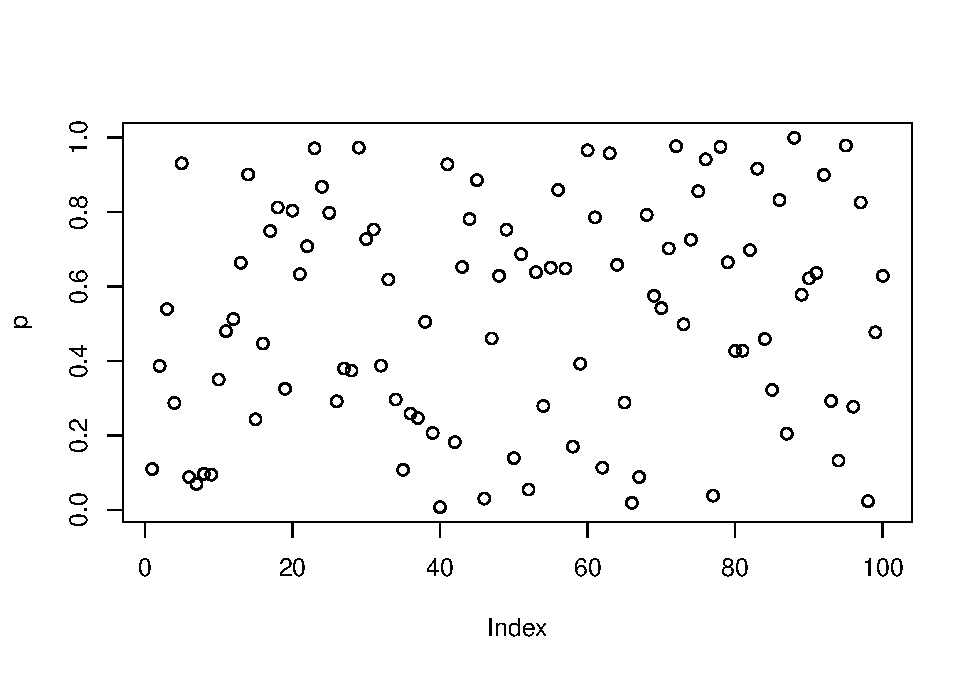
\includegraphics{Functionals_files/figure-latex/unnamed-chunk-7-1.pdf}

\hypertarget{q5.-fixing-non-functioning-code}{%
\subsection*{Q5. Fixing non-functioning code}\label{q5.-fixing-non-functioning-code}}
\addcontentsline{toc}{subsection}{Q5. Fixing non-functioning code}

\begin{Shaded}
\begin{Highlighting}[]
\NormalTok{x }\OtherTok{\textless{}{-}} \FunctionTok{list}\NormalTok{(}
  \FunctionTok{list}\NormalTok{(}\DecValTok{1}\NormalTok{, }\FunctionTok{c}\NormalTok{(}\DecValTok{3}\NormalTok{, }\DecValTok{9}\NormalTok{)),}
  \FunctionTok{list}\NormalTok{(}\FunctionTok{c}\NormalTok{(}\DecValTok{3}\NormalTok{, }\DecValTok{6}\NormalTok{), }\DecValTok{7}\NormalTok{, }\FunctionTok{c}\NormalTok{(}\DecValTok{4}\NormalTok{, }\DecValTok{7}\NormalTok{, }\DecValTok{6}\NormalTok{))}
\NormalTok{)}

\NormalTok{triple }\OtherTok{\textless{}{-}} \ControlFlowTok{function}\NormalTok{(x) x }\SpecialCharTok{*} \DecValTok{3}
\FunctionTok{map}\NormalTok{(x, }\AttributeTok{.f =} \SpecialCharTok{\textasciitilde{}} \FunctionTok{map}\NormalTok{(., }\SpecialCharTok{\textasciitilde{}} \FunctionTok{triple}\NormalTok{(.)))}
\CommentTok{\#\textgreater{} [[1]]}
\CommentTok{\#\textgreater{} [[1]][[1]]}
\CommentTok{\#\textgreater{} [1] 3}
\CommentTok{\#\textgreater{} }
\CommentTok{\#\textgreater{} [[1]][[2]]}
\CommentTok{\#\textgreater{} [1]  9 27}
\CommentTok{\#\textgreater{} }
\CommentTok{\#\textgreater{} }
\CommentTok{\#\textgreater{} [[2]]}
\CommentTok{\#\textgreater{} [[2]][[1]]}
\CommentTok{\#\textgreater{} [1]  9 18}
\CommentTok{\#\textgreater{} }
\CommentTok{\#\textgreater{} [[2]][[2]]}
\CommentTok{\#\textgreater{} [1] 21}
\CommentTok{\#\textgreater{} }
\CommentTok{\#\textgreater{} [[2]][[3]]}
\CommentTok{\#\textgreater{} [1] 12 21 18}
\end{Highlighting}
\end{Shaded}

\hypertarget{q6.-use-map-to-fit-linear-models-to-the-mtcars-dataset}{%
\subsection*{\texorpdfstring{Q6. Use \texttt{map()} to fit linear models to the \texttt{mtcars} dataset}{Q6. Use map() to fit linear models to the mtcars dataset}}\label{q6.-use-map-to-fit-linear-models-to-the-mtcars-dataset}}
\addcontentsline{toc}{subsection}{Q6. Use \texttt{map()} to fit linear models to the \texttt{mtcars} dataset}

\begin{Shaded}
\begin{Highlighting}[]
\NormalTok{formulas }\OtherTok{\textless{}{-}} \FunctionTok{list}\NormalTok{(}
\NormalTok{  mpg }\SpecialCharTok{\textasciitilde{}}\NormalTok{ disp,}
\NormalTok{  mpg }\SpecialCharTok{\textasciitilde{}} \FunctionTok{I}\NormalTok{(}\DecValTok{1} \SpecialCharTok{/}\NormalTok{ disp),}
\NormalTok{  mpg }\SpecialCharTok{\textasciitilde{}}\NormalTok{ disp }\SpecialCharTok{+}\NormalTok{ wt,}
\NormalTok{  mpg }\SpecialCharTok{\textasciitilde{}} \FunctionTok{I}\NormalTok{(}\DecValTok{1} \SpecialCharTok{/}\NormalTok{ disp) }\SpecialCharTok{+}\NormalTok{ wt}
\NormalTok{)}

\FunctionTok{map}\NormalTok{(formulas, }\SpecialCharTok{\textasciitilde{}} \FunctionTok{lm}\NormalTok{(}\AttributeTok{formula =}\NormalTok{ ., }\AttributeTok{data =}\NormalTok{ mtcars))}
\CommentTok{\#\textgreater{} [[1]]}
\CommentTok{\#\textgreater{} }
\CommentTok{\#\textgreater{} Call:}
\CommentTok{\#\textgreater{} lm(formula = ., data = mtcars)}
\CommentTok{\#\textgreater{} }
\CommentTok{\#\textgreater{} Coefficients:}
\CommentTok{\#\textgreater{} (Intercept)         disp  }
\CommentTok{\#\textgreater{}    29.59985     {-}0.04122  }
\CommentTok{\#\textgreater{} }
\CommentTok{\#\textgreater{} }
\CommentTok{\#\textgreater{} [[2]]}
\CommentTok{\#\textgreater{} }
\CommentTok{\#\textgreater{} Call:}
\CommentTok{\#\textgreater{} lm(formula = ., data = mtcars)}
\CommentTok{\#\textgreater{} }
\CommentTok{\#\textgreater{} Coefficients:}
\CommentTok{\#\textgreater{} (Intercept)    I(1/disp)  }
\CommentTok{\#\textgreater{}       10.75      1557.67  }
\CommentTok{\#\textgreater{} }
\CommentTok{\#\textgreater{} }
\CommentTok{\#\textgreater{} [[3]]}
\CommentTok{\#\textgreater{} }
\CommentTok{\#\textgreater{} Call:}
\CommentTok{\#\textgreater{} lm(formula = ., data = mtcars)}
\CommentTok{\#\textgreater{} }
\CommentTok{\#\textgreater{} Coefficients:}
\CommentTok{\#\textgreater{} (Intercept)         disp           wt  }
\CommentTok{\#\textgreater{}    34.96055     {-}0.01772     {-}3.35083  }
\CommentTok{\#\textgreater{} }
\CommentTok{\#\textgreater{} }
\CommentTok{\#\textgreater{} [[4]]}
\CommentTok{\#\textgreater{} }
\CommentTok{\#\textgreater{} Call:}
\CommentTok{\#\textgreater{} lm(formula = ., data = mtcars)}
\CommentTok{\#\textgreater{} }
\CommentTok{\#\textgreater{} Coefficients:}
\CommentTok{\#\textgreater{} (Intercept)    I(1/disp)           wt  }
\CommentTok{\#\textgreater{}      19.024     1142.560       {-}1.798}
\end{Highlighting}
\end{Shaded}

\hypertarget{q7.-computing-r-squared}{%
\subsection*{Q7. Computing R-squared}\label{q7.-computing-r-squared}}
\addcontentsline{toc}{subsection}{Q7. Computing R-squared}

\begin{Shaded}
\begin{Highlighting}[]
\NormalTok{bootstrap }\OtherTok{\textless{}{-}} \ControlFlowTok{function}\NormalTok{(df) \{}
\NormalTok{  df[}\FunctionTok{sample}\NormalTok{(}\FunctionTok{nrow}\NormalTok{(df), }\AttributeTok{replace =} \ConstantTok{TRUE}\NormalTok{), , drop }\OtherTok{=} \ConstantTok{FALSE}\NormalTok{]}
\NormalTok{\}}

\NormalTok{bootstraps }\OtherTok{\textless{}{-}} \FunctionTok{map}\NormalTok{(}\DecValTok{1}\SpecialCharTok{:}\DecValTok{10}\NormalTok{, }\SpecialCharTok{\textasciitilde{}} \FunctionTok{bootstrap}\NormalTok{(mtcars))}

\FunctionTok{map\_dbl}\NormalTok{(}
\NormalTok{  bootstraps,}
  \SpecialCharTok{\textasciitilde{}} \FunctionTok{summary}\NormalTok{(}\FunctionTok{lm}\NormalTok{(}\AttributeTok{formula =}\NormalTok{ mpg }\SpecialCharTok{\textasciitilde{}}\NormalTok{ disp, }\AttributeTok{data =}\NormalTok{ .))}\SpecialCharTok{$}\NormalTok{r.squared}
\NormalTok{)}
\CommentTok{\#\textgreater{}  [1] 0.7467027 0.7839514 0.7263799 0.7319638 0.7652060}
\CommentTok{\#\textgreater{}  [6] 0.7377944 0.7204561 0.7430256 0.8514938 0.7326552}
\end{Highlighting}
\end{Shaded}

\hypertarget{exercise-9.4.6}{%
\section{Exercise 9.4.6}\label{exercise-9.4.6}}

\hypertarget{q1.-explain-the-results}{%
\subsection*{Q1. Explain the results}\label{q1.-explain-the-results}}
\addcontentsline{toc}{subsection}{Q1. Explain the results}

\texttt{modify()} returns the object of type same as the input. Since the input here is a dataframe of certain dimensions and \texttt{.f\ =\ 1} translates to plucking the first element in each column, it returns a dataframes with the same dimensions with the plucked element recycled across rows.

\begin{Shaded}
\begin{Highlighting}[]
\FunctionTok{head}\NormalTok{(}\FunctionTok{modify}\NormalTok{(mtcars, }\DecValTok{1}\NormalTok{))}
\CommentTok{\#\textgreater{}                   mpg cyl disp  hp drat   wt  qsec vs am}
\CommentTok{\#\textgreater{} Mazda RX4          21   6  160 110  3.9 2.62 16.46  0  1}
\CommentTok{\#\textgreater{} Mazda RX4 Wag      21   6  160 110  3.9 2.62 16.46  0  1}
\CommentTok{\#\textgreater{} Datsun 710         21   6  160 110  3.9 2.62 16.46  0  1}
\CommentTok{\#\textgreater{} Hornet 4 Drive     21   6  160 110  3.9 2.62 16.46  0  1}
\CommentTok{\#\textgreater{} Hornet Sportabout  21   6  160 110  3.9 2.62 16.46  0  1}
\CommentTok{\#\textgreater{} Valiant            21   6  160 110  3.9 2.62 16.46  0  1}
\CommentTok{\#\textgreater{}                   gear carb}
\CommentTok{\#\textgreater{} Mazda RX4            4    4}
\CommentTok{\#\textgreater{} Mazda RX4 Wag        4    4}
\CommentTok{\#\textgreater{} Datsun 710           4    4}
\CommentTok{\#\textgreater{} Hornet 4 Drive       4    4}
\CommentTok{\#\textgreater{} Hornet Sportabout    4    4}
\CommentTok{\#\textgreater{} Valiant              4    4}
\end{Highlighting}
\end{Shaded}

\hypertarget{q2.-use-iwalk-instead-of-walk2}{%
\subsection*{\texorpdfstring{Q2. Use \texttt{iwalk()} instead of \texttt{walk2()}}{Q2. Use iwalk() instead of walk2()}}\label{q2.-use-iwalk-instead-of-walk2}}
\addcontentsline{toc}{subsection}{Q2. Use \texttt{iwalk()} instead of \texttt{walk2()}}

\begin{Shaded}
\begin{Highlighting}[]
\CommentTok{\# with walk2() {-}{-}{-}{-}{-}{-}{-}{-}{-}{-}{-}{-}{-}{-}{-}{-}{-}{-}{-}{-}{-}{-}{-}}

\NormalTok{cyls }\OtherTok{\textless{}{-}} \FunctionTok{split}\NormalTok{(mtcars, mtcars}\SpecialCharTok{$}\NormalTok{cyl)}
\NormalTok{paths }\OtherTok{\textless{}{-}} \FunctionTok{file.path}\NormalTok{(temp, }\FunctionTok{paste0}\NormalTok{(}\StringTok{"cyl{-}"}\NormalTok{, }\FunctionTok{names}\NormalTok{(cyls), }\StringTok{".csv"}\NormalTok{))}
\FunctionTok{walk2}\NormalTok{(}\AttributeTok{.x =}\NormalTok{ cyls, }\AttributeTok{.y =}\NormalTok{ paths, }\AttributeTok{.f =}\NormalTok{ write.csv)}

\CommentTok{\# with iwalk {-}{-}{-}{-}{-}{-}{-}{-}{-}{-}{-}{-}{-}{-}{-}{-}{-}{-}{-}{-}{-}{-}{-}{-}{-}{-}}

\NormalTok{cyls }\OtherTok{\textless{}{-}} \FunctionTok{split}\NormalTok{(mtcars, mtcars}\SpecialCharTok{$}\NormalTok{cyl)}
\FunctionTok{names}\NormalTok{(cyls) }\OtherTok{\textless{}{-}} \FunctionTok{file.path}\NormalTok{(temp, }\FunctionTok{paste0}\NormalTok{(}\StringTok{"cyl{-}"}\NormalTok{, }\FunctionTok{names}\NormalTok{(cyls), }\StringTok{".csv"}\NormalTok{))}
\FunctionTok{iwalk}\NormalTok{(cyls, }\SpecialCharTok{\textasciitilde{}} \FunctionTok{write.csv}\NormalTok{(.x, .y))}
\end{Highlighting}
\end{Shaded}

\hypertarget{q3.-explain-the-code}{%
\subsection*{Q3. Explain the code}\label{q3.-explain-the-code}}
\addcontentsline{toc}{subsection}{Q3. Explain the code}

\texttt{map2()} supplies the functions defined in \texttt{.x\ =\ trans} as \texttt{f} in the anonymous functions, while the names of the columns defined in \texttt{.y\ =\ mtcars{[}nm{]}} are picked up by \texttt{var} in the anonymous function. Note that the function is iterating over indices for vectors of transformations and column names.

\begin{Shaded}
\begin{Highlighting}[]
\NormalTok{trans }\OtherTok{\textless{}{-}} \FunctionTok{list}\NormalTok{(}
  \AttributeTok{disp =} \ControlFlowTok{function}\NormalTok{(x) x }\SpecialCharTok{*} \FloatTok{0.0163871}\NormalTok{,}
  \AttributeTok{am =} \ControlFlowTok{function}\NormalTok{(x) }\FunctionTok{factor}\NormalTok{(x, }\AttributeTok{labels =} \FunctionTok{c}\NormalTok{(}\StringTok{"auto"}\NormalTok{, }\StringTok{"manual"}\NormalTok{))}
\NormalTok{)}

\NormalTok{nm }\OtherTok{\textless{}{-}} \FunctionTok{names}\NormalTok{(trans)}
\NormalTok{mtcars[nm] }\OtherTok{\textless{}{-}} \FunctionTok{map2}\NormalTok{(trans, mtcars[nm], }\ControlFlowTok{function}\NormalTok{(f, var) }\FunctionTok{f}\NormalTok{(var))}
\end{Highlighting}
\end{Shaded}

In the \texttt{map} approach, the function is iterating over indices for vectors of column names.

\begin{Shaded}
\begin{Highlighting}[]
\NormalTok{mtcars[nm] }\OtherTok{\textless{}{-}} \FunctionTok{map}\NormalTok{(nm, }\SpecialCharTok{\textasciitilde{}}\NormalTok{ trans[[.x]](mtcars[[.x]]))}
\end{Highlighting}
\end{Shaded}

\hypertarget{q4.-difference-between-map2-and-walk2}{%
\subsection*{\texorpdfstring{Q4. Difference between \texttt{map2()} and \texttt{walk2()}}{Q4. Difference between map2() and walk2()}}\label{q4.-difference-between-map2-and-walk2}}
\addcontentsline{toc}{subsection}{Q4. Difference between \texttt{map2()} and \texttt{walk2()}}

If we use \texttt{map2()}, it will work, but it will print \texttt{NULL} to the terminal for every element of the list.

\begin{Shaded}
\begin{Highlighting}[]
\NormalTok{bods }\OtherTok{\textless{}{-}} \FunctionTok{split}\NormalTok{(BOD, BOD}\SpecialCharTok{$}\NormalTok{Time)}
\NormalTok{nm }\OtherTok{\textless{}{-}} \FunctionTok{names}\NormalTok{(bods)}
\FunctionTok{map2}\NormalTok{(bods, nm, write.csv)}
\end{Highlighting}
\end{Shaded}

\hypertarget{exercise-9.6.3}{%
\section{Exercise 9.6.3}\label{exercise-9.6.3}}

\hypertarget{q1.-predicate-functions}{%
\subsection*{Q1. Predicate functions}\label{q1.-predicate-functions}}
\addcontentsline{toc}{subsection}{Q1. Predicate functions}

\begin{quote}
A predicate is a function that returns a \textbf{single} \texttt{TRUE} or \texttt{FALSE}.
\end{quote}

The \texttt{is.na()} function does not return a single value, but instead returns a vector and thus isn't a predicate function.

\begin{Shaded}
\begin{Highlighting}[]
\CommentTok{\# contrast the following behavior of predicate functions}
\FunctionTok{is.character}\NormalTok{(}\FunctionTok{c}\NormalTok{(}\StringTok{"x"}\NormalTok{, }\DecValTok{2}\NormalTok{))}
\CommentTok{\#\textgreater{} [1] TRUE}
\FunctionTok{is.null}\NormalTok{(}\FunctionTok{c}\NormalTok{(}\DecValTok{3}\NormalTok{, }\ConstantTok{NULL}\NormalTok{))}
\CommentTok{\#\textgreater{} [1] FALSE}

\CommentTok{\# with this behavior}
\FunctionTok{is.na}\NormalTok{(}\FunctionTok{c}\NormalTok{(}\ConstantTok{NA}\NormalTok{, }\DecValTok{1}\NormalTok{))}
\CommentTok{\#\textgreater{} [1]  TRUE FALSE}
\end{Highlighting}
\end{Shaded}

The closest equivalent of a predicate function in base-R is \texttt{anyNA()} function.

\begin{Shaded}
\begin{Highlighting}[]
\FunctionTok{anyNA}\NormalTok{(}\FunctionTok{c}\NormalTok{(}\ConstantTok{NA}\NormalTok{, }\DecValTok{1}\NormalTok{))}
\CommentTok{\#\textgreater{} [1] TRUE}
\end{Highlighting}
\end{Shaded}

\hypertarget{q2.-fix-simple_reduce}{%
\subsection*{\texorpdfstring{Q2. Fix \texttt{simple\_reduce}}{Q2. Fix simple\_reduce}}\label{q2.-fix-simple_reduce}}
\addcontentsline{toc}{subsection}{Q2. Fix \texttt{simple\_reduce}}

Supplied function:

\begin{Shaded}
\begin{Highlighting}[]
\NormalTok{simple\_reduce }\OtherTok{\textless{}{-}} \ControlFlowTok{function}\NormalTok{(x, f) \{}
\NormalTok{  out }\OtherTok{\textless{}{-}}\NormalTok{ x[[}\DecValTok{1}\NormalTok{]]}
  \ControlFlowTok{for}\NormalTok{ (i }\ControlFlowTok{in} \FunctionTok{seq}\NormalTok{(}\DecValTok{2}\NormalTok{, }\FunctionTok{length}\NormalTok{(x))) \{}
\NormalTok{    out }\OtherTok{\textless{}{-}} \FunctionTok{f}\NormalTok{(out, x[[i]])}
\NormalTok{  \}}
\NormalTok{  out}
\NormalTok{\}}
\end{Highlighting}
\end{Shaded}

Struggles with inputs of length 0 and 1 because function tries to access out-of-bound values.

\begin{Shaded}
\begin{Highlighting}[]
\FunctionTok{simple\_reduce}\NormalTok{(}\FunctionTok{numeric}\NormalTok{(), sum)}
\CommentTok{\#\textgreater{} Error in x[[1]]: subscript out of bounds}
\FunctionTok{simple\_reduce}\NormalTok{(}\DecValTok{1}\NormalTok{, sum)}
\CommentTok{\#\textgreater{} Error in x[[i]]: subscript out of bounds}
\FunctionTok{simple\_reduce}\NormalTok{(}\DecValTok{1}\SpecialCharTok{:}\DecValTok{3}\NormalTok{, sum)}
\CommentTok{\#\textgreater{} [1] 6}
\end{Highlighting}
\end{Shaded}

This problem can be solved by adding \texttt{init} argument, which supplies the default or initial value for the function to operate on:

\begin{Shaded}
\begin{Highlighting}[]
\NormalTok{simple\_reduce2 }\OtherTok{\textless{}{-}} \ControlFlowTok{function}\NormalTok{(x, f, }\AttributeTok{init =} \DecValTok{0}\NormalTok{) \{}
  \CommentTok{\# initializer will become the first value}
  \ControlFlowTok{if}\NormalTok{ (}\FunctionTok{length}\NormalTok{(x) }\SpecialCharTok{==}\NormalTok{ 0L) \{}
    \FunctionTok{return}\NormalTok{(init)}
\NormalTok{  \}}
  \ControlFlowTok{if}\NormalTok{ (}\FunctionTok{length}\NormalTok{(x) }\SpecialCharTok{==}\NormalTok{ 1L) \{}
    \FunctionTok{return}\NormalTok{(x[[1L]])}
\NormalTok{  \}}

\NormalTok{  out }\OtherTok{\textless{}{-}}\NormalTok{ x[[}\DecValTok{1}\NormalTok{]]}

  \ControlFlowTok{for}\NormalTok{ (i }\ControlFlowTok{in} \FunctionTok{seq}\NormalTok{(}\DecValTok{2}\NormalTok{, }\FunctionTok{length}\NormalTok{(x))) \{}
\NormalTok{    out }\OtherTok{\textless{}{-}} \FunctionTok{f}\NormalTok{(out, x[[i]])}
\NormalTok{  \}}
\NormalTok{  out}
\NormalTok{\}}
\end{Highlighting}
\end{Shaded}

Let's try it out:

\begin{Shaded}
\begin{Highlighting}[]
\FunctionTok{simple\_reduce2}\NormalTok{(}\FunctionTok{numeric}\NormalTok{(), sum)}
\CommentTok{\#\textgreater{} [1] 0}
\FunctionTok{simple\_reduce2}\NormalTok{(}\DecValTok{1}\NormalTok{, sum)}
\CommentTok{\#\textgreater{} [1] 1}
\FunctionTok{simple\_reduce2}\NormalTok{(}\DecValTok{1}\SpecialCharTok{:}\DecValTok{3}\NormalTok{, sum)}
\CommentTok{\#\textgreater{} [1] 6}
\end{Highlighting}
\end{Shaded}

With a different kind of function:

\begin{Shaded}
\begin{Highlighting}[]
\FunctionTok{simple\_reduce2}\NormalTok{(}\FunctionTok{numeric}\NormalTok{(), }\StringTok{\textasciigrave{}}\AttributeTok{*}\StringTok{\textasciigrave{}}\NormalTok{, }\AttributeTok{init =} \DecValTok{1}\NormalTok{)}
\CommentTok{\#\textgreater{} [1] 1}
\FunctionTok{simple\_reduce2}\NormalTok{(}\DecValTok{1}\NormalTok{, }\StringTok{\textasciigrave{}}\AttributeTok{*}\StringTok{\textasciigrave{}}\NormalTok{, }\AttributeTok{init =} \DecValTok{1}\NormalTok{)}
\CommentTok{\#\textgreater{} [1] 1}
\FunctionTok{simple\_reduce2}\NormalTok{(}\DecValTok{1}\SpecialCharTok{:}\DecValTok{3}\NormalTok{, }\StringTok{\textasciigrave{}}\AttributeTok{*}\StringTok{\textasciigrave{}}\NormalTok{, }\AttributeTok{init =} \DecValTok{1}\NormalTok{)}
\CommentTok{\#\textgreater{} [1] 6}
\end{Highlighting}
\end{Shaded}

And another one:

\begin{Shaded}
\begin{Highlighting}[]
\FunctionTok{simple\_reduce2}\NormalTok{(}\FunctionTok{numeric}\NormalTok{(), }\StringTok{\textasciigrave{}}\AttributeTok{\%/\%}\StringTok{\textasciigrave{}}\NormalTok{)}
\CommentTok{\#\textgreater{} [1] 0}
\FunctionTok{simple\_reduce2}\NormalTok{(}\DecValTok{1}\NormalTok{, }\StringTok{\textasciigrave{}}\AttributeTok{\%/\%}\StringTok{\textasciigrave{}}\NormalTok{)}
\CommentTok{\#\textgreater{} [1] 1}
\FunctionTok{simple\_reduce2}\NormalTok{(}\DecValTok{1}\SpecialCharTok{:}\DecValTok{3}\NormalTok{, }\StringTok{\textasciigrave{}}\AttributeTok{\%/\%}\StringTok{\textasciigrave{}}\NormalTok{)}
\CommentTok{\#\textgreater{} [1] 0}
\end{Highlighting}
\end{Shaded}

\hypertarget{exercise-9.7.3}{%
\section{Exercise 9.7.3}\label{exercise-9.7.3}}

\hypertarget{q1.}{%
\subsection*{Q1.}\label{q1.}}
\addcontentsline{toc}{subsection}{Q1.}

\hypertarget{q2.-eapply-and-rapply}{%
\subsection*{\texorpdfstring{Q2. \texttt{eapply()} and \texttt{rapply()}}{Q2. eapply() and rapply()}}\label{q2.-eapply-and-rapply}}
\addcontentsline{toc}{subsection}{Q2. \texttt{eapply()} and \texttt{rapply()}}

\begin{quote}
\texttt{eapply()} applies FUN to the named values from an environment and returns the results as a list.
\end{quote}

\begin{quote}
\texttt{rapply()} is a recursive version of lapply with flexibility in how the result is structured (how = ``..'').
\end{quote}

\hypertarget{s3}{%
\chapter{S3}\label{s3}}

\hypertarget{exercise-13.2.1}{%
\section{Exercise 13.2.1}\label{exercise-13.2.1}}

\hypertarget{q1.-differences-between-t.test-and-t.data.frame}{%
\subsection*{\texorpdfstring{Q1. Differences between \texttt{t.test} and \texttt{t.data.frame}}{Q1. Differences between t.test and t.data.frame}}\label{q1.-differences-between-t.test-and-t.data.frame}}
\addcontentsline{toc}{subsection}{Q1. Differences between \texttt{t.test} and \texttt{t.data.frame}}

\begin{Shaded}
\begin{Highlighting}[]
\FunctionTok{library}\NormalTok{(sloop)}

\CommentTok{\# function type}
\FunctionTok{ftype}\NormalTok{(t.test)}
\CommentTok{\#\textgreater{} [1] "S3"      "generic"}
\FunctionTok{ftype}\NormalTok{(t.data.frame)}
\CommentTok{\#\textgreater{} [1] "S3"     "method"}
\end{Highlighting}
\end{Shaded}

\begin{itemize}
\item
  \texttt{t.test()} is a \textbf{generic} function to perform t-test.
\item
  \texttt{t.data.frame} is a \textbf{method} for generic \texttt{t()} (a matrix transform function) and will be dispatched for \texttt{data.frame} objects that need to be transformed.
\end{itemize}

\hypertarget{q2.-base-r-function-with-.}{%
\subsection*{\texorpdfstring{Q2. base-R function with \texttt{.}}{Q2. base-R function with .}}\label{q2.-base-r-function-with-.}}
\addcontentsline{toc}{subsection}{Q2. base-R function with \texttt{.}}

\begin{itemize}
\tightlist
\item
  \texttt{all.equal()}
\item
  Most of \texttt{as.*} functions like \texttt{as.data.frame()}
\item
  \texttt{install.packages()}
  etc.
\end{itemize}

For example,

\begin{Shaded}
\begin{Highlighting}[]
\FunctionTok{ftype}\NormalTok{(as.data.frame)}
\CommentTok{\#\textgreater{} [1] "S3"      "generic"}
\end{Highlighting}
\end{Shaded}

\hypertarget{q3.-what-does-as.data.frame.data.frame-do}{%
\subsection*{\texorpdfstring{Q3. What does \texttt{as.data.frame.data.frame()} do?}{Q3. What does as.data.frame.data.frame() do?}}\label{q3.-what-does-as.data.frame.data.frame-do}}
\addcontentsline{toc}{subsection}{Q3. What does \texttt{as.data.frame.data.frame()} do?}

It's a \textbf{method} for generic \texttt{as.data.frame()}.

Less confusing: \texttt{asDataFrame.DataFrame()}.

\hypertarget{q4.-difference-in-behavior}{%
\subsection*{Q4. Difference in behavior}\label{q4.-difference-in-behavior}}
\addcontentsline{toc}{subsection}{Q4. Difference in behavior}

Before unclassing, the S3 dispatches \texttt{.Date} method, while after \texttt{.numeric} method.

Before

\begin{Shaded}
\begin{Highlighting}[]
\NormalTok{some\_days }\OtherTok{\textless{}{-}} \FunctionTok{as.Date}\NormalTok{(}\StringTok{"2017{-}01{-}31"}\NormalTok{) }\SpecialCharTok{+} \FunctionTok{sample}\NormalTok{(}\DecValTok{10}\NormalTok{, }\DecValTok{5}\NormalTok{)}

\NormalTok{some\_days}
\CommentTok{\#\textgreater{} [1] "2017{-}02{-}09" "2017{-}02{-}03" "2017{-}02{-}04" "2017{-}02{-}01"}
\CommentTok{\#\textgreater{} [5] "2017{-}02{-}10"}

\FunctionTok{s3\_dispatch}\NormalTok{(}\FunctionTok{mean}\NormalTok{(some\_days))}
\CommentTok{\#\textgreater{} =\textgreater{} mean.Date}
\CommentTok{\#\textgreater{}  * mean.default}

\FunctionTok{mean}\NormalTok{(some\_days)}
\CommentTok{\#\textgreater{} [1] "2017{-}02{-}05"}
\end{Highlighting}
\end{Shaded}

After

\begin{Shaded}
\begin{Highlighting}[]
\FunctionTok{unclass}\NormalTok{(some\_days)}
\CommentTok{\#\textgreater{} [1] 17206 17200 17201 17198 17207}

\FunctionTok{mean}\NormalTok{(}\FunctionTok{unclass}\NormalTok{(some\_days))}
\CommentTok{\#\textgreater{} [1] 17202.4}

\FunctionTok{s3\_dispatch}\NormalTok{(}\FunctionTok{mean}\NormalTok{(}\FunctionTok{unclass}\NormalTok{(some\_days)))}
\CommentTok{\#\textgreater{}    mean.double}
\CommentTok{\#\textgreater{}    mean.numeric}
\CommentTok{\#\textgreater{} =\textgreater{} mean.default}
\end{Highlighting}
\end{Shaded}

\hypertarget{q5.-object-properties}{%
\subsection*{Q5. Object properties}\label{q5.-object-properties}}
\addcontentsline{toc}{subsection}{Q5. Object properties}

\begin{Shaded}
\begin{Highlighting}[]
\NormalTok{x }\OtherTok{\textless{}{-}} \FunctionTok{ecdf}\NormalTok{(}\FunctionTok{rpois}\NormalTok{(}\DecValTok{100}\NormalTok{, }\DecValTok{10}\NormalTok{))}
\NormalTok{x}
\CommentTok{\#\textgreater{} Empirical CDF }
\CommentTok{\#\textgreater{} Call: ecdf(rpois(100, 10))}
\CommentTok{\#\textgreater{}  x[1:14] =      4,      5,      6,  ...,     16,     17}

\FunctionTok{otype}\NormalTok{(x)}
\CommentTok{\#\textgreater{} [1] "S3"}

\FunctionTok{attributes}\NormalTok{(x)}
\CommentTok{\#\textgreater{} $class}
\CommentTok{\#\textgreater{} [1] "ecdf"     "stepfun"  "function"}
\CommentTok{\#\textgreater{} }
\CommentTok{\#\textgreater{} $call}
\CommentTok{\#\textgreater{} ecdf(rpois(100, 10))}

\FunctionTok{s3\_class}\NormalTok{(x)}
\CommentTok{\#\textgreater{} [1] "ecdf"     "stepfun"  "function"}
\end{Highlighting}
\end{Shaded}

\hypertarget{q6.-object-properties}{%
\subsection*{Q6. Object properties}\label{q6.-object-properties}}
\addcontentsline{toc}{subsection}{Q6. Object properties}

\begin{Shaded}
\begin{Highlighting}[]
\NormalTok{x }\OtherTok{\textless{}{-}} \FunctionTok{table}\NormalTok{(}\FunctionTok{rpois}\NormalTok{(}\DecValTok{100}\NormalTok{, }\DecValTok{5}\NormalTok{))}
\NormalTok{x}
\CommentTok{\#\textgreater{} }
\CommentTok{\#\textgreater{}  0  1  2  3  4  5  6  7  8  9 10 11 12 }
\CommentTok{\#\textgreater{}  1  4 10 12 16 22  9 15  4  2  3  1  1}

\FunctionTok{otype}\NormalTok{(x)}
\CommentTok{\#\textgreater{} [1] "S3"}

\FunctionTok{attributes}\NormalTok{(x)}
\CommentTok{\#\textgreater{} $dim}
\CommentTok{\#\textgreater{} [1] 13}
\CommentTok{\#\textgreater{} }
\CommentTok{\#\textgreater{} $dimnames}
\CommentTok{\#\textgreater{} $dimnames[[1]]}
\CommentTok{\#\textgreater{}  [1] "0"  "1"  "2"  "3"  "4"  "5"  "6"  "7"  "8"  "9"  "10"}
\CommentTok{\#\textgreater{} [12] "11" "12"}
\CommentTok{\#\textgreater{} }
\CommentTok{\#\textgreater{} }
\CommentTok{\#\textgreater{} $class}
\CommentTok{\#\textgreater{} [1] "table"}

\FunctionTok{s3\_class}\NormalTok{(x)}
\CommentTok{\#\textgreater{} [1] "table"}
\end{Highlighting}
\end{Shaded}

\hypertarget{r6}{%
\chapter{R6}\label{r6}}

\hypertarget{exercise-14.2.6}{%
\section{Exercise 14.2.6}\label{exercise-14.2.6}}

\hypertarget{q1.-r6-class-for-bank-account}{%
\subsection*{Q1. R6 class for bank account}\label{q1.-r6-class-for-bank-account}}
\addcontentsline{toc}{subsection}{Q1. R6 class for bank account}

Create the superclass and make sure it works as expected.

\begin{Shaded}
\begin{Highlighting}[]
\FunctionTok{library}\NormalTok{(R6)}

\CommentTok{\# define the needed class}
\NormalTok{bankAccount }\OtherTok{\textless{}{-}}\NormalTok{ R6}\SpecialCharTok{::}\FunctionTok{R6Class}\NormalTok{(}
  \StringTok{"bankAccount"}\NormalTok{,}
  \AttributeTok{public =} \FunctionTok{list}\NormalTok{(}
    \CommentTok{\# fields {-}{-}{-}{-}{-}{-}{-}{-}{-}{-}{-}{-}{-}{-}{-}{-}{-}{-}{-}{-}{-}{-}{-}}
    \AttributeTok{balance =} \ConstantTok{NA}\NormalTok{,}
    \AttributeTok{name =} \ConstantTok{NA}\NormalTok{,}

    \CommentTok{\# methods {-}{-}{-}{-}{-}{-}{-}{-}{-}{-}{-}{-}{-}{-}{-}{-}{-}{-}{-}{-}{-}{-}}
    \AttributeTok{initialize =} \ControlFlowTok{function}\NormalTok{(}\AttributeTok{name =} \ConstantTok{NULL}\NormalTok{, balance) \{}
\NormalTok{      self}\SpecialCharTok{$}\FunctionTok{validate}\NormalTok{(balance)}

\NormalTok{      self}\SpecialCharTok{$}\NormalTok{name }\OtherTok{\textless{}{-}}\NormalTok{ name}
\NormalTok{      self}\SpecialCharTok{$}\NormalTok{balance }\OtherTok{\textless{}{-}}\NormalTok{ balance}
\NormalTok{    \},}
    \AttributeTok{deposit =} \ControlFlowTok{function}\NormalTok{(amount) \{}
\NormalTok{      self}\SpecialCharTok{$}\FunctionTok{validate}\NormalTok{(amount)}
      \FunctionTok{cat}\NormalTok{(}\StringTok{"Current balance is: "}\NormalTok{, self}\SpecialCharTok{$}\NormalTok{balance, }\StringTok{"}\SpecialCharTok{\textbackslash{}n}\StringTok{"}\NormalTok{, }\AttributeTok{sep =} \StringTok{""}\NormalTok{)}
      \FunctionTok{cat}\NormalTok{(}\StringTok{"And you are depositing: "}\NormalTok{, amount)}
\NormalTok{      self}\SpecialCharTok{$}\NormalTok{balance }\OtherTok{\textless{}{-}}\NormalTok{ self}\SpecialCharTok{$}\NormalTok{balance }\SpecialCharTok{+}\NormalTok{ amount}
      \FunctionTok{invisible}\NormalTok{(self)}
\NormalTok{    \},}
    \AttributeTok{withdraw =} \ControlFlowTok{function}\NormalTok{(amount) \{}
\NormalTok{      self}\SpecialCharTok{$}\FunctionTok{validate}\NormalTok{(amount)}
      \FunctionTok{cat}\NormalTok{(}\StringTok{"Current balance is: "}\NormalTok{, self}\SpecialCharTok{$}\NormalTok{balance, }\StringTok{"}\SpecialCharTok{\textbackslash{}n}\StringTok{"}\NormalTok{, }\AttributeTok{sep =} \StringTok{""}\NormalTok{)}
      \FunctionTok{cat}\NormalTok{(}\StringTok{"And you are withdrawing: "}\NormalTok{, amount, }\StringTok{"}\SpecialCharTok{\textbackslash{}n}\StringTok{"}\NormalTok{, }\AttributeTok{sep =} \StringTok{""}\NormalTok{)}
\NormalTok{      self}\SpecialCharTok{$}\NormalTok{balance }\OtherTok{\textless{}{-}}\NormalTok{ self}\SpecialCharTok{$}\NormalTok{balance }\SpecialCharTok{{-}}\NormalTok{ amount}
      \FunctionTok{invisible}\NormalTok{(self)}
\NormalTok{    \},}
    \AttributeTok{validate =} \ControlFlowTok{function}\NormalTok{(amount) \{}
      \FunctionTok{stopifnot}\NormalTok{(}\FunctionTok{is.numeric}\NormalTok{(amount), amount }\SpecialCharTok{\textgreater{}=} \DecValTok{0}\NormalTok{)}
\NormalTok{    \},}
    \AttributeTok{print =} \ControlFlowTok{function}\NormalTok{() \{}
      \FunctionTok{cat}\NormalTok{(}\StringTok{"Dear "}\NormalTok{, self}\SpecialCharTok{$}\NormalTok{name, }\StringTok{", your balance is: "}\NormalTok{, self}\SpecialCharTok{$}\NormalTok{balance, }\AttributeTok{sep =} \StringTok{""}\NormalTok{)}
      \FunctionTok{invisible}\NormalTok{(self)}
\NormalTok{    \}}
\NormalTok{  )}
\NormalTok{)}

\CommentTok{\# create an instance of an object}
\NormalTok{indra }\OtherTok{\textless{}{-}}\NormalTok{ bankAccount}\SpecialCharTok{$}\FunctionTok{new}\NormalTok{(}\AttributeTok{name =} \StringTok{"Indra"}\NormalTok{, }\AttributeTok{balance =} \DecValTok{100}\NormalTok{)}

\NormalTok{indra}
\CommentTok{\#\textgreater{} Dear Indra, your balance is: 100}

\CommentTok{\# do deposits and withdrawals to see if the balance changes}
\NormalTok{indra}\SpecialCharTok{$}\FunctionTok{deposit}\NormalTok{(}\DecValTok{20}\NormalTok{)}
\CommentTok{\#\textgreater{} Current balance is: 100}
\CommentTok{\#\textgreater{} And you are depositing:  20}

\NormalTok{indra}
\CommentTok{\#\textgreater{} Dear Indra, your balance is: 120}

\NormalTok{indra}\SpecialCharTok{$}\FunctionTok{withdraw}\NormalTok{(}\DecValTok{10}\NormalTok{)}
\CommentTok{\#\textgreater{} Current balance is: 120}
\CommentTok{\#\textgreater{} And you are withdrawing: 10}

\NormalTok{indra}
\CommentTok{\#\textgreater{} Dear Indra, your balance is: 110}

\CommentTok{\# make sure input validation checks work}
\NormalTok{indra}\SpecialCharTok{$}\FunctionTok{deposit}\NormalTok{(}\SpecialCharTok{{-}}\DecValTok{20}\NormalTok{)}
\CommentTok{\#\textgreater{} Error in self$validate(amount): amount \textgreater{}= 0 is not TRUE}
\NormalTok{indra}\SpecialCharTok{$}\FunctionTok{deposit}\NormalTok{(}\StringTok{"pizza"}\NormalTok{)}
\CommentTok{\#\textgreater{} Error in self$validate(amount): is.numeric(amount) is not TRUE}
\NormalTok{indra}\SpecialCharTok{$}\FunctionTok{withdraw}\NormalTok{(}\SpecialCharTok{{-}}\DecValTok{54}\NormalTok{)}
\CommentTok{\#\textgreater{} Error in self$validate(amount): amount \textgreater{}= 0 is not TRUE}
\NormalTok{Anne }\OtherTok{\textless{}{-}}\NormalTok{ bankAccount}\SpecialCharTok{$}\FunctionTok{new}\NormalTok{(}\AttributeTok{name =} \StringTok{"Anne"}\NormalTok{, }\AttributeTok{balance =} \SpecialCharTok{{-}}\DecValTok{45}\NormalTok{)}
\CommentTok{\#\textgreater{} Error in self$validate(balance): amount \textgreater{}= 0 is not TRUE}
\end{Highlighting}
\end{Shaded}

Create a subclass that errors if you attempt to overdraw

\begin{Shaded}
\begin{Highlighting}[]
\NormalTok{bankAccountStrict }\OtherTok{\textless{}{-}}\NormalTok{ R6}\SpecialCharTok{::}\FunctionTok{R6Class}\NormalTok{(}
  \StringTok{"bankAccountStrict"}\NormalTok{,}
  \AttributeTok{inherit =}\NormalTok{ bankAccount,}
  \AttributeTok{public =} \FunctionTok{list}\NormalTok{(}
    \AttributeTok{withdraw =} \ControlFlowTok{function}\NormalTok{(amount) \{}
      \CommentTok{\# use method from superclass}
\NormalTok{      super}\SpecialCharTok{$}\FunctionTok{withdraw}\NormalTok{(amount)}

      \ControlFlowTok{if}\NormalTok{ (self}\SpecialCharTok{$}\NormalTok{balance }\SpecialCharTok{\textless{}} \DecValTok{0}\NormalTok{) \{}
        \FunctionTok{invisible}\NormalTok{(self)}
        \FunctionTok{stop}\NormalTok{(}
          \FunctionTok{cat}\NormalTok{(}\StringTok{"}\SpecialCharTok{\textbackslash{}n}\StringTok{You are trying to withdraw more that your balance.}\SpecialCharTok{\textbackslash{}n}\StringTok{"}\NormalTok{),}
          \FunctionTok{cat}\NormalTok{(}\StringTok{"I\textquotesingle{}m sorry, "}\NormalTok{, self}\SpecialCharTok{$}\NormalTok{name, }\StringTok{", I\textquotesingle{}m afraid I can\textquotesingle{}t do that."}\NormalTok{, }\AttributeTok{sep =} \StringTok{""}\NormalTok{),}
          \AttributeTok{call. =} \ConstantTok{FALSE}
\NormalTok{        )}
\NormalTok{      \}}
\NormalTok{    \}}
\NormalTok{  )}
\NormalTok{)}

\CommentTok{\# create an instance of an object}
\NormalTok{Pritesh }\OtherTok{\textless{}{-}}\NormalTok{ bankAccountStrict}\SpecialCharTok{$}\FunctionTok{new}\NormalTok{(}\AttributeTok{name =} \StringTok{"Pritesh"}\NormalTok{, }\AttributeTok{balance =} \DecValTok{100}\NormalTok{)}

\NormalTok{Pritesh}
\CommentTok{\#\textgreater{} Dear Pritesh, your balance is: 100}

\CommentTok{\# do deposits and withdrawals to see if the balance changes}
\NormalTok{Pritesh}\SpecialCharTok{$}\FunctionTok{deposit}\NormalTok{(}\DecValTok{20}\NormalTok{)}
\CommentTok{\#\textgreater{} Current balance is: 100}
\CommentTok{\#\textgreater{} And you are depositing:  20}

\NormalTok{Pritesh}
\CommentTok{\#\textgreater{} Dear Pritesh, your balance is: 120}

\NormalTok{Pritesh}\SpecialCharTok{$}\FunctionTok{withdraw}\NormalTok{(}\DecValTok{150}\NormalTok{)}
\CommentTok{\#\textgreater{} Current balance is: 120}
\CommentTok{\#\textgreater{} And you are withdrawing: 150}
\CommentTok{\#\textgreater{} }
\CommentTok{\#\textgreater{} You are trying to withdraw more that your balance.}
\CommentTok{\#\textgreater{} I\textquotesingle{}m sorry, Pritesh, I\textquotesingle{}m afraid I can\textquotesingle{}t do that.}
\CommentTok{\#\textgreater{} Error:}

\NormalTok{Pritesh}
\CommentTok{\#\textgreater{} Dear Pritesh, your balance is: {-}30}

\CommentTok{\# make sure input validation checks work}
\NormalTok{Pritesh}\SpecialCharTok{$}\FunctionTok{deposit}\NormalTok{(}\SpecialCharTok{{-}}\DecValTok{20}\NormalTok{)}
\CommentTok{\#\textgreater{} Error in self$validate(amount): amount \textgreater{}= 0 is not TRUE}
\NormalTok{Pritesh}\SpecialCharTok{$}\FunctionTok{deposit}\NormalTok{(}\StringTok{"pizza"}\NormalTok{)}
\CommentTok{\#\textgreater{} Error in self$validate(amount): is.numeric(amount) is not TRUE}
\NormalTok{Pritesh}\SpecialCharTok{$}\FunctionTok{withdraw}\NormalTok{(}\SpecialCharTok{{-}}\DecValTok{54}\NormalTok{)}
\CommentTok{\#\textgreater{} Error in self$validate(amount): amount \textgreater{}= 0 is not TRUE}
\NormalTok{Pritesh }\OtherTok{\textless{}{-}}\NormalTok{ bankAccountStrict}\SpecialCharTok{$}\FunctionTok{new}\NormalTok{(}\AttributeTok{name =} \StringTok{"Pritesh"}\NormalTok{, }\AttributeTok{balance =} \SpecialCharTok{{-}}\DecValTok{45}\NormalTok{)}
\CommentTok{\#\textgreater{} Error in self$validate(balance): amount \textgreater{}= 0 is not TRUE}
\end{Highlighting}
\end{Shaded}

Create a subclass that charges a fee if overdraw

\begin{Shaded}
\begin{Highlighting}[]
\NormalTok{bankAccountFee }\OtherTok{\textless{}{-}}\NormalTok{ R6}\SpecialCharTok{::}\FunctionTok{R6Class}\NormalTok{(}
  \StringTok{"bankAccountFee"}\NormalTok{,}
  \AttributeTok{inherit =}\NormalTok{ bankAccount,}
  \AttributeTok{public =} \FunctionTok{list}\NormalTok{(}
    \AttributeTok{withdraw =} \ControlFlowTok{function}\NormalTok{(amount) \{}
      \CommentTok{\# use method from superclass}
\NormalTok{      super}\SpecialCharTok{$}\FunctionTok{withdraw}\NormalTok{(amount)}

      \ControlFlowTok{if}\NormalTok{ (self}\SpecialCharTok{$}\NormalTok{balance }\SpecialCharTok{\textless{}} \DecValTok{0}\NormalTok{) \{}
        \FunctionTok{cat}\NormalTok{(}\StringTok{"}\SpecialCharTok{\textbackslash{}n}\StringTok{I am charging you 10 euros for overdrawing.}\SpecialCharTok{\textbackslash{}n}\StringTok{"}\NormalTok{)}
\NormalTok{        self}\SpecialCharTok{$}\NormalTok{balance }\OtherTok{\textless{}{-}}\NormalTok{ self}\SpecialCharTok{$}\NormalTok{balance }\SpecialCharTok{{-}} \DecValTok{10}
        \FunctionTok{invisible}\NormalTok{(self)}
\NormalTok{      \}}
\NormalTok{    \}}
\NormalTok{  )}
\NormalTok{)}

\CommentTok{\# create an instance of an object}
\NormalTok{Mangesh }\OtherTok{\textless{}{-}}\NormalTok{ bankAccountFee}\SpecialCharTok{$}\FunctionTok{new}\NormalTok{(}\AttributeTok{name =} \StringTok{"Mangesh"}\NormalTok{, }\AttributeTok{balance =} \DecValTok{100}\NormalTok{)}

\NormalTok{Mangesh}
\CommentTok{\#\textgreater{} Dear Mangesh, your balance is: 100}

\CommentTok{\# do deposits and withdrawals to see if the balance changes}
\NormalTok{Mangesh}\SpecialCharTok{$}\FunctionTok{deposit}\NormalTok{(}\DecValTok{20}\NormalTok{)}
\CommentTok{\#\textgreater{} Current balance is: 100}
\CommentTok{\#\textgreater{} And you are depositing:  20}

\NormalTok{Mangesh}
\CommentTok{\#\textgreater{} Dear Mangesh, your balance is: 120}

\NormalTok{Mangesh}\SpecialCharTok{$}\FunctionTok{withdraw}\NormalTok{(}\DecValTok{150}\NormalTok{)}
\CommentTok{\#\textgreater{} Current balance is: 120}
\CommentTok{\#\textgreater{} And you are withdrawing: 150}
\CommentTok{\#\textgreater{} }
\CommentTok{\#\textgreater{} I am charging you 10 euros for overdrawing.}

\NormalTok{Mangesh}
\CommentTok{\#\textgreater{} Dear Mangesh, your balance is: {-}40}

\CommentTok{\# make sure input validation checks work}
\NormalTok{Mangesh}\SpecialCharTok{$}\FunctionTok{deposit}\NormalTok{(}\SpecialCharTok{{-}}\DecValTok{20}\NormalTok{)}
\CommentTok{\#\textgreater{} Error in self$validate(amount): amount \textgreater{}= 0 is not TRUE}
\NormalTok{Mangesh}\SpecialCharTok{$}\FunctionTok{deposit}\NormalTok{(}\StringTok{"pizza"}\NormalTok{)}
\CommentTok{\#\textgreater{} Error in self$validate(amount): is.numeric(amount) is not TRUE}
\NormalTok{Mangesh}\SpecialCharTok{$}\FunctionTok{withdraw}\NormalTok{(}\SpecialCharTok{{-}}\DecValTok{54}\NormalTok{)}
\CommentTok{\#\textgreater{} Error in self$validate(amount): amount \textgreater{}= 0 is not TRUE}
\NormalTok{Mangesh }\OtherTok{\textless{}{-}}\NormalTok{ bankAccountFee}\SpecialCharTok{$}\FunctionTok{new}\NormalTok{(}\AttributeTok{name =} \StringTok{"Mangesh"}\NormalTok{, }\AttributeTok{balance =} \SpecialCharTok{{-}}\DecValTok{45}\NormalTok{)}
\CommentTok{\#\textgreater{} Error in self$validate(balance): amount \textgreater{}= 0 is not TRUE}
\end{Highlighting}
\end{Shaded}

\hypertarget{q2.-r6-class-for-carddeck}{%
\subsection*{Q2. R6 class for carddeck}\label{q2.-r6-class-for-carddeck}}
\addcontentsline{toc}{subsection}{Q2. R6 class for carddeck}

\begin{Shaded}
\begin{Highlighting}[]
\NormalTok{suit }\OtherTok{\textless{}{-}} \FunctionTok{c}\NormalTok{(}\StringTok{"SPADE"}\NormalTok{, }\StringTok{"HEARTS"}\NormalTok{, }\StringTok{"DIAMOND"}\NormalTok{, }\StringTok{"CLUB"}\NormalTok{) }\CommentTok{\# sigh, Windows encoding issues}
\NormalTok{value }\OtherTok{\textless{}{-}} \FunctionTok{c}\NormalTok{(}\StringTok{"A"}\NormalTok{, }\DecValTok{2}\SpecialCharTok{:}\DecValTok{10}\NormalTok{, }\StringTok{"J"}\NormalTok{, }\StringTok{"Q"}\NormalTok{, }\StringTok{"K"}\NormalTok{)}
\NormalTok{cards }\OtherTok{\textless{}{-}} \FunctionTok{paste}\NormalTok{(}\FunctionTok{rep}\NormalTok{(value, }\DecValTok{4}\NormalTok{), suit)}

\NormalTok{deck }\OtherTok{\textless{}{-}}\NormalTok{ R6}\SpecialCharTok{::}\FunctionTok{R6Class}\NormalTok{(}
  \StringTok{"deck"}\NormalTok{,}
  \AttributeTok{public =} \FunctionTok{list}\NormalTok{(}
    \CommentTok{\# fields {-}{-}{-}{-}{-}{-}{-}{-}{-}{-}{-}{-}{-}{-}{-}{-}{-}{-}{-}{-}{-}{-}{-}}

    \CommentTok{\# methods {-}{-}{-}{-}{-}{-}{-}{-}{-}{-}{-}{-}{-}{-}{-}{-}{-}{-}{-}{-}{-}{-}{-}}
    \AttributeTok{draw =} \ControlFlowTok{function}\NormalTok{(n) \{}
      \FunctionTok{sample}\NormalTok{(self}\SpecialCharTok{$}\NormalTok{cards, n)}
\NormalTok{    \},}
    \AttributeTok{reshuffle =} \ControlFlowTok{function}\NormalTok{() \{}
      \FunctionTok{sample}\NormalTok{(self}\SpecialCharTok{$}\NormalTok{cards)}
      \FunctionTok{invisible}\NormalTok{(self)}
\NormalTok{    \},}
    \AttributeTok{print =} \ControlFlowTok{function}\NormalTok{() \{}
      \StringTok{"Drawn cards are:"}
      \StringTok{"Number of remaining cards:"}
\NormalTok{    \}}
\NormalTok{  )}
\NormalTok{)}

\CommentTok{\# create a new instance of this object}
\NormalTok{mydeck }\OtherTok{\textless{}{-}}\NormalTok{ deck}\SpecialCharTok{$}\FunctionTok{new}\NormalTok{()}

\CommentTok{\# draw cards}
\NormalTok{mydeck}\SpecialCharTok{$}\FunctionTok{draw}\NormalTok{(}\DecValTok{4}\NormalTok{)}

\CommentTok{\# reshuffle}
\end{Highlighting}
\end{Shaded}

\hypertarget{big-picture}{%
\chapter{Big Picture}\label{big-picture}}

No exercises.

  \bibliography{book.bib,packages.bib}

\end{document}
